\documentclass{article}

\usepackage{silence}              % load first: suppress the benign \showhyphens redefinition notice
\WarningFilter{latex}{Command}      % kernel \CheckCommand emits "Command \showhyphens has changed."
\WarningFilter{microtype}{Command}
\usepackage[T1]{fontenc}
\usepackage[utf8]{inputenc}   % if you're using UTF-8

\usepackage{graphicx} % Required for inserting images
\usepackage{multirow}
\usepackage{booktabs}
\usepackage{array}
\usepackage{amsmath}
\usepackage{enumerate}
\usepackage{caption}
\usepackage{float}
\usepackage[title,titletoc]{appendix}
\usepackage{hyperref}
\usepackage{xurl}        % allow URLs (e.g. the \url in the bibliography) to break anywhere -> no overfull line
\usepackage{subcaption}  % for subfigures
\usepackage{tikz}        % scoring-modes schematic
\usetikzlibrary{arrows.meta, positioning, fit, backgrounds}
\usepackage{cite}        % numeric IEEE-style citation grouping
\usepackage[bottom=3cm, right=3cm, left=3cm, top=3cm]{geometry}
\usepackage{microtype}            % char protrusion + font expansion: clears sub-line overfulls
\setlength{\emergencystretch}{3em} % last-resort interword stretch: removes residual overfull \hbox
\setlength{\hfuzz}{1pt}             % ignore sub-pixel (<1pt) overfulls
\usepackage{etoolbox}
\AtBeginEnvironment{thebibliography}{\sloppy} % standard: loosen line-breaking in the bibliography
\hypersetup{                       % explicit PDF metadata so hyperref never derives strings from the rich \title
    pdftitle={Open-Vocabulary Temporal Change Retrieval},
    pdfauthor={Panagiotis Giannikos and Markos Syroukis}
}

% Figures live under figures/ (including the NTUA logo).
\graphicspath{{figures/}{images/}}


\author{}
\title{
    {
\includegraphics[width=3cm]{figures/NTUA-logo.png}}\par
    {\Large NATIONAL TECHNICAL UNIVERSITY OF ATHENS} \par \vspace{0.2cm}
    % {\large SCHOOL OF ELECTRICAL AND COMPUTER ENGINEERING \par \vspace{0.5cm}
    % IPPS DATA SCIENCE AND MACHINE LEARNING \par \vspace{0.5cm}
    {\large GEOSPATIAL BIG DATA ANALYTICS  \par \vspace{0.5cm}
    Professors: K. Karantzalos, V. Douskos, V. Tsironis, A. Psalta \par \vspace{0.5cm}
    Students:\\Panagiotis Giannikos, panagiotisgiannikos@mail.ntua.gr, 03400245, IPPS Data Science and Machine Learning \par
    Markos Syroukis, ma.siroukis@gmail.com, 09325023, IPPS Mathematical Modeling \par \vspace{0.5cm}}
    {\Large Open-Vocabulary Temporal Change Retrieval}
    \par \vspace{-1cm}
    }
\date{}



\begin{document}

\maketitle


\phantomsection
\addcontentsline{toc}{section}{Abstract}
\section*{Abstract}

We build a semantic change search engine that, given a free-text query
(e.g. ``agricultural land converted to wetland''), ranks bi-temporal
satellite image pairs by how well the change between the two timesteps
matches the query, and returns the matched tiles, the timestep, a localisation
heatmap, a match score, and a seasonal-vs-permanent flag. A query may name a
change \emph{type} -- a property of the later state, such as ``a new road'' --
or a directional change \emph{transition} such as the example above, and the two
are best served by different scoring approaches. The system uses
frozen CLIP-variant vision-language backbones and compares three
scoring approaches - a naive image baseline, a zero-shot $\Delta$-similarity,
and a parameter-efficient fine-tuned (PEFT) adapter - across three encoders
on Dynamic EarthNet (DEN), with three further datasets (QFabric, LEVIR-CC/MCI,
and SECOND-CC) validating the dataset-agnostic design and extending it to
open-vocabulary breadth and pixel-level change localisation. All findings are
reported under a strict statistical protocol (random-ranking baselines, FDR
correction, and leave-one-AOI-out cross-validation). Out of distribution, the
frozen zero-shot score beats the learned PEFT and LoRA adapters: the adapters'
high in-distribution scores (0.420--0.999 mAP) measure the adapter evaluated on
its own training pairs (memorisation) and collapse to or below chance on
held-out areas. Single-split test mAP on the 110-pair split is high-variance -
the GeoRSCLIP+NRG configuration reaches 0.426 on one split, while its 5-fold AOI
cross-validated estimate is $0.100 \pm 0.139$. Defining retrieval relevance by
the per-class pixel-fraction change the labels already encode, and scoring
change locally with a patch-level $\Delta$-score, raises cross-validated mAP to
$0.193 \pm 0.051$ and makes localised change-types - new buildings and urban
expansion, with new water borderline - retrievable above chance. On LEVIR-CC (a
public benchmark of human-captioned building-change pairs) the same frozen engine
retrieves salient building and road change strongly
(per-query AP $\approx$0.6--0.8) but subtle vegetation and sparse water change
only near their prevalence floors, so the open-vocabulary signal scales sharply
with change salience. SECOND-CC extends this to a seven-query open vocabulary -
every change type clears its prevalence floor but only modestly (zero-shot macro
$\approx$0.33 vs a $\approx$0.30 floor). Using the LEVIR-MCI and SECOND-CC pixel masks we
also score the change heatmap quantitatively: it is a weak localiser
(pointing-game lift within $\pm$0.04--0.10 of a random-patch floor), so
localising change is harder than retrieving it. The recurring lesson is that
spectral physics and spatial locality carry what signal exists, while global
embeddings and learned visual priors dilute or memorise it -- and that
single-split scores must be cross-validated before they estimate generalisation.


\setcounter{tocdepth}{2}
\tableofcontents


\clearpage


\section{Introduction and objectives}
\label{sec:intro}

Traditional change detection is limited to a few predefined categories
(e.g. ``urban growth'' or ``forest loss'')~\cite{changedetection}. This project
moves toward open-vocabulary change retrieval by leveraging Vision-Language
Models (VLMs)~\cite{clip}: instead of training a class-specific detector, we
build a system that identifies semantically defined transitions from
natural-language queries (e.g. ``new industrial buildings appearing on former
agricultural land'') and searches across a multitemporal dataset to find the
tiles and time-steps where the described change occurred. Text and image-change
embeddings are aligned, and a pair is scored by the cosine similarity between
its change embedding and the query embedding.

Per the GBDA Lab Project's general guidelines, the work is constrained to a low-compute budget and
must deliver a subset of an appropriate dataset, CLIP-variant frozen encoders,
both zero-shot inference and light PEFT, retrieval metrics (Recall@$K$, mAP), an
error analysis of seasonal-vs-permanent confusion (``semantic drift''), and a
Gradio~\cite{gradio} Semantic Change Search Engine as the product deliverable.
The primary dataset is Dynamic EarthNet (DEN)~\cite{dynamicearthnet}, which
provides daily multi-spectral Planet Fusion~\cite{planetfusion} data ideal for
pinpointing the exact time-step of change (evaluated in
Appendix~\ref{sec:temporalpinpoint}); the dataset-agnostic design is
exercised on QFabric~\cite{qfabric}, LEVIR-CC/MCI~\cite{levircc,levirmci}, and
SECOND-CC~\cite{secondcc}.

This report makes three contributions. First, it delivers a working,
dataset-agnostic open-vocabulary change-retrieval engine with a Gradio interface
and a label-grounded Recall@$K$/mAP benchmark. Second, it reports a careful,
statistically audited comparison of frozen zero-shot scoring against light
parameter-efficient fine-tuning across three CLIP-variant encoders, three colour
modes, and four datasets, with leave-one-AOI-out cross-validation as the
generalisation estimate. Third, it identifies and characterises a single
organising principle that holds across every dataset: the recovered change
signal scales with the spatial and semantic \emph{salience} of the change. We
state this salience hypothesis at the outset - salient, well-described
construction change is retrievable, while subtle, sparse, or rare transitions
collapse toward their prevalence floor - and test it systematically. The
companion findings are that frozen RS-pretrained features with NIR false-colour
and localised patch scoring carry what weak signal exists, and that low-compute
fine-tuning does not improve retrieval out of distribution.

The remainder of this report covers the theoretical background
(Section~\ref{sec:background}), related work (Section~\ref{sec:related}), the
system architecture (Section~\ref{sec:arch}), the retrieval approaches and
scoring (Section~\ref{sec:methods}), the data and encoders
(Section~\ref{sec:data}), the evaluation protocol and metrics
(Section~\ref{sec:eval}), the experiments and results
(Section~\ref{sec:results}), resources and operational metrics
(Section~\ref{sec:resources}), reproducibility (Section~\ref{sec:repro}),
limitations and future work (Section~\ref{sec:future}), and conclusions
(Section~\ref{sec:conclusion}).


\section{Background and theory}
\label{sec:background}

\paragraph{Change detection: types and transitions.}
Remote-sensing change detection has classically estimated, per pixel or per
region, whether and how land cover changed between two co-registered
acquisitions~\cite{changedetection}. Two questions are distinct and recur
throughout this report. A change \emph{type} is a property of the later state
(``this is now a road''), recoverable from the after-image alone; a change
\emph{transition} is directional (``cleared land became a building''), and
requires comparing both timesteps. Open-vocabulary retrieval generalises the
classical setting by replacing a fixed label set with free-text queries, so the
same engine must serve both questions; which scoring rule wins depends on which
question a query asks.

\paragraph{Contrastive vision-language models.}
CLIP~\cite{clip} and its open reproduction OpenCLIP~\cite{openclip} train a dual
encoder - a vision tower (here a Vision Transformer~\cite{vit}) and a text
tower - so that matching image--text pairs have high cosine similarity -- the dot
product of the $L_2$-normalised embeddings, $\cos(u,v)=u\cdot v/(\lVert u\rVert\,
\lVert v\rVert)\in[-1,1]$, with $1$ meaning identical direction -- in a shared
embedding space, using a contrastive InfoNCE~\cite{infonce} objective over large
web corpora. Because the space is
shared and normalised, an unseen text query can be scored against an image by
cosine similarity with no task-specific training; this is the zero-shot transfer
property the engine relies on. We exploit it twice: directly (the after-image
score) and on a change feature built from the two timesteps' embeddings.

\paragraph{Remote-sensing foundation models and the domain gap.}
General web-pretrained CLIP embeds everyday scene appearance, which need not
align with overhead multi-spectral imagery or with subtle land-cover
transitions; this is a distribution-shift problem, and zero-shot transfer is
known to degrade under natural shift~\cite{distshift}. RS-specialised
contrastive models narrow the gap by continuing contrastive pre-training on
remote-sensing image--text data: GeoRSCLIP~\cite{georsclip} on the large RS5M
corpus, and RemoteCLIP~\cite{remoteclip} on curated RS caption data. A central
empirical question of this report is whether such domain pre-training, or
light task adaptation, materially closes the gap for temporal change retrieval.

\paragraph{Parameter-efficient fine-tuning.}
When a frozen backbone underperforms, the low-compute alternative to full
fine-tuning is to train a small number of added parameters. Adapter
modules~\cite{peftadapters} insert tiny trainable bottlenecks while freezing the
backbone; LoRA~\cite{lora} instead learns low-rank updates to existing weight
matrices, adding well under 1\% of parameters. We use both: a small
projection-head adapter over the change feature, and LoRA on the visual
encoder's feed-forward projections. PEFT trades capacity for lower
catastrophic-forgetting risk and compute; as the results show, limited capacity
does not by itself prevent memorising a small training set.

\paragraph{Spectral background: NIR false-colour.}
Vegetation reflects strongly in the near-infrared and absorbs in the red, the
basis of vegetation indices such as NDVI~\cite{vegindex}. Mapping
NIR-Red-Green into the three input channels (an ``NRG'' false-colour) therefore
exposes vegetation and moisture contrasts that an RGB composite suppresses,
which matters for the agriculture$\leftrightarrow$wetland transitions that
dominate the primary dataset. The Planet Fusion~\cite{planetfusion} and
Sentinel-2~\cite{sentinel2} sensors both carry the requisite NIR band.

\paragraph{Retrieval metrics and the statistical protocol.}
Retrieval quality is measured with standard information-retrieval
metrics~\cite{irmetrics}: for each query, average precision (AP) summarises the
ranked list, mean average precision (mAP) macro-averages AP over queries, and
Recall@$K$ is the fraction of relevant items in the top $K$. Two properties
shape their interpretation here. A random ranker scores mAP equal to the query's
prevalence (its positive fraction), so mAP is read against a prevalence floor,
not against zero; and Recall@$K$ is upper-bounded by $K/R$ when the relevant set
$R$ is large, so it is read for ordering rather than absolute height. Because
single small splits are high-variance, we estimate generalisation with $k$-fold
\emph{leave-one-AOI-out} cross-validation, which partitions by geographic area
of interest so that no area appears in both train and evaluation, controlling
the leakage that otherwise inflates learned adapters. Significance is assessed
against a Monte-Carlo random-ranking baseline (a permutation test~\cite{permtest}
on the ranking with the relevant set fixed), with bootstrap~\cite{bootstrap}
confidence intervals and
Benjamini--Hochberg~\cite{benjaminihochberg} false-discovery-rate correction
across the query set. Localisation of the change heatmap is scored with the
pointing-game metric~\cite{pointinggame} - whether the most-activated patch
falls on a true change region - and patch-level AP, each against a random-patch
floor.


\section{Related work}
\label{sec:related}

\paragraph{RS vision-language foundation models.}
GeoRSCLIP~\cite{georsclip} and RemoteCLIP~\cite{remoteclip} adapt the CLIP recipe
to remote sensing and are the domain backbones evaluated here; both target
scene-level image--text alignment rather than temporal change, which is precisely
the gap this project probes. Temporal earth-observation assistants such as
TEOChat~\cite{teochat} pair imagery with instruction-style temporal questions; we
reuse its QFabric question--answer annotations as a label source while keeping a
lightweight retrieval engine rather than a generative assistant.

\paragraph{Change-captioning datasets.}
LEVIR-CC~\cite{levircc} pairs bi-temporal building-change scenes with human
captions; LEVIR-MCI~\cite{levirmci} adds pixel-level change masks over the same
pairs; SECOND-CC~\cite{secondcc} pairs captions with six-class
SECOND~\cite{second} semantic maps for a far wider land-cover vocabulary. We use
these not as captioning benchmarks but as open-vocabulary retrieval and
localisation testbeds with caption- and mask-grounded relevance. The primary
dataset, DynamicEarthNet~\cite{dynamicearthnet}, contributes dense daily
multi-spectral imagery with monthly land-cover labels, which is what makes
exact-timestep change retrieval possible; QFabric~\cite{qfabric} and
fMoW~\cite{fmow} contribute construction-centric and functional change taxonomies
respectively.

\paragraph{Positioning.}
Against this body of work, the engine here is deliberately frozen-backbone and
low-compute: it asks how far zero-shot scoring and light PEFT carry
open-vocabulary change retrieval across four datasets under an honest statistical
audit, rather than proposing a new trained change model. The reusable
contribution is the dataset-agnostic protocol and the salience-scaled reading of
when frozen VLM features succeed.


\section{System architecture}
\label{sec:arch}

For each bi-temporal pair $(T_1, T_2)$ the pipeline proceeds as follows. A frozen
VLM encodes both timesteps into $L_2$-normalised global embeddings
$f_{T_1}, f_{T_2}$, cached to disk per (dataset, encoder, split, colour mode).
A change feature is then formed, either as a difference
$\Delta f = f_{T_2} - f_{T_1}$ or as a concatenation $[f_{T_1} ; f_{T_2}]$. The
query text is encoded by the same model's text tower into $t$, and the pair is
scored by one of the approaches of Section~\ref{sec:methods}.
Figure~\ref{fig:engine-pipeline} summarises the engine end to end.

\begin{figure}[H]
    \centering
    
\includegraphics[width=\linewidth]{engine_pipeline.png}
    \caption{Open-vocabulary temporal change-retrieval engine. A frozen CLIP-variant encoder
    (CLIP ViT-L/14, GeoRSCLIP, or RemoteCLIP; optionally with a light LoRA/PEFT head) embeds the
    text query and both timesteps; a pair is scored by global $\Delta$-similarity or by the localised
    \texttt{patch\_top3} change score (the best Dynamic EarthNet configuration); pairs are ranked into
    the top-$K$ change events, each surfaced in the Gradio app as a $T_1/T_2$ side-by-side with a
    query-conditioned change heatmap and a match score in $[0,1]$. A seasonal-drift gate filters
    stable-pair false positives.}
    \label{fig:engine-pipeline}
\end{figure}

\paragraph{Dataset-agnostic core.}
A structural \texttt{TemporalDataset} protocol defines the only contract
downstream code depends on: list the locations and bi-temporal pairs, load the
images, load metadata, and derive a ground-truth change label. A registry maps a
dataset name to a loader, and one concrete loader per dataset and on-disk format
implements that contract -- for Dynamic EarthNet (both the preprocessed 24-month
arrays and the monthly rasters), for QFabric (polygon-centred crops carrying the
real change-type labels benchmarked in Section~\ref{sec:crossdataset}, plus a
status-transition sibling), and for the captioned, mask-annotated LEVIR-CC,
LEVIR-MCI, and SECOND-CC. Adding a dataset or encoder means adding a file, never
editing the shared pipeline: the abstraction is enforced by the protocol, and the
full source is in the linked repository.

\paragraph{Encoders.}
An \texttt{ImageTextEncoder} protocol (\texttt{src/encoders/base.py}) has three
implementations: \texttt{clip\_vitl14} (HuggingFace CLIP~\cite{clip} on a
ViT~\cite{vit} backbone, 768-d), \texttt{georsclip}
(\texttt{open\_clip}~\cite{openclip} ViT-B/32 + RS5M checkpoint~\cite{georsclip},
512-d), and \texttt{remoteclip} (\texttt{open\_clip} ViT-L/14 + RemoteCLIP
checkpoint~\cite{remoteclip}, 768-d). All backbones are frozen and run in
evaluation mode; the embedding dimension drives cache and index sizing
automatically.

\paragraph{PEFT training.}
Only the \texttt{ProjectionHead} adapter trains; the backbones stay frozen.
Supervision is DEN's weak caption derived from its land-use / land-cover (LULC)
labels (e.g. ``agriculture replaced by wetlands'', ``stable forest land cover''). The
loss is a masked symmetric InfoNCE~\cite{infonce}: pairs sharing an identical
caption are treated as mutual positives~\cite{supcon}, which avoids the
false-negative problem of plain diagonal InfoNCE, since DEN captions repeat heavily.

\paragraph{Search engine.}
Evaluation is label-grounded against a fixed query set, and the same scoring path
drives the Gradio Semantic Change Search Engine. A user types a free-text query
(for example ``new buildings or houses constructed''); the engine scores every
bi-temporal pair in the loaded corpus, ranks them, and returns the top change
events. Each event shows the $T_1$ (before) and $T_2$ (after) image side by side,
a query-conditioned change heatmap highlighting where in the tile the queried
change is strongest, a match score in $[0,1]$, and a seasonal-vs-permanent note
that flags pairs whose difference is driven by seasonal or illumination drift
rather than persistent change. The match score is the raw retrieval score
(Section~\ref{sec:methods}) min--max normalised across the returned set: it ranks
results relative to one another within a single query and is not a calibrated
probability. The heatmap is the per-patch query-conditioned $\Delta$-similarity
field of Section~\ref{sec:methods}, normalised the same way. Two optional
re-ranking toggles (location diversity and geographic coherence) and a continental
filter aid exploratory browsing. A snapshot is shown in Figure~\ref{fig:app}.

\begin{figure}[H]
    \centering
    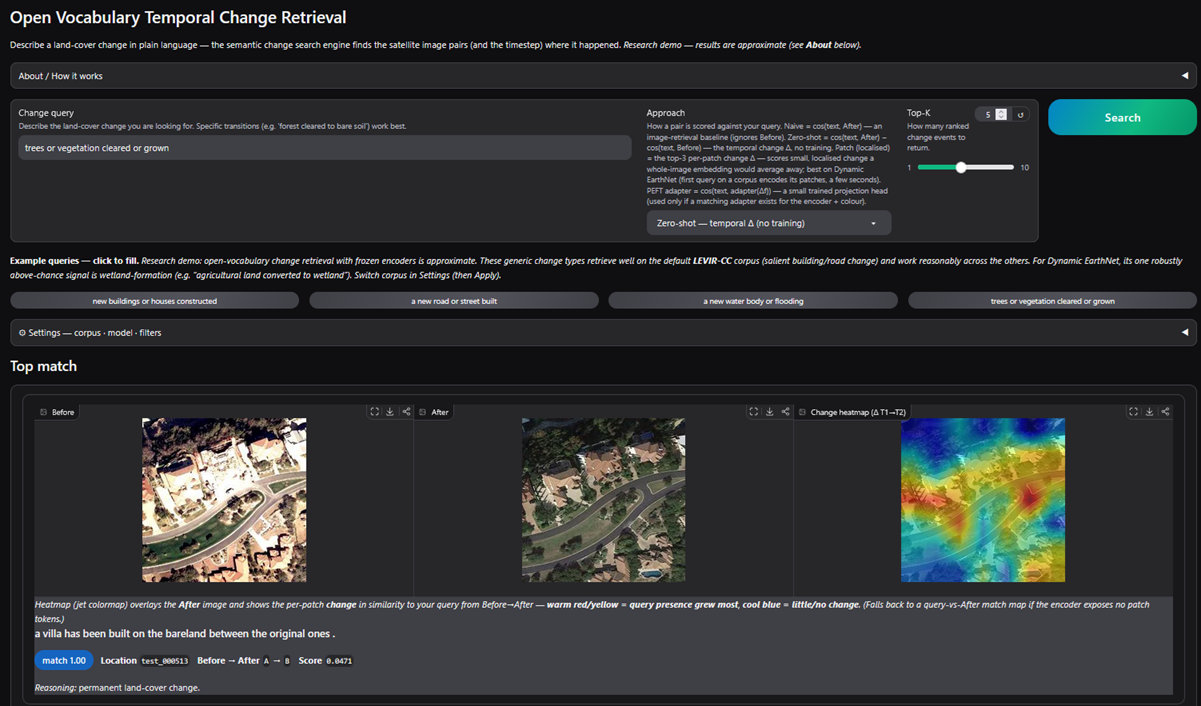
\includegraphics[width=\linewidth]{app_screenshot.png}
    \caption{The deployed Gradio Semantic Change Search Engine. A free-text query
    returns a ranked list of change events; the top match is inspected through
    interactive before/after and after/heatmap comparison sliders, and the remaining
    matches through a thumbnail grid with per-result inspect controls, each result
    carrying a match score and a seasonal-vs-permanent note.}
    \label{fig:app}
\end{figure}


\section{Retrieval approaches and scoring}
\label{sec:methods}

Three global-embedding approaches are compared end-to-end, and a localised
patch-level scorer is added on top. Let $t$ be the $L_2$-normalised query
embedding and $f_{T_1}, f_{T_2}$ the $L_2$-normalised image embeddings of the
two timesteps. The global scores are:

\begin{align}
    s_{\text{naive}}     &= \cos\!\big(t,\, f_{T_2}\big) && \text{(image-retrieval lower bound; no training)} \\
    s_{\text{zero\_shot}} &= \cos\!\big(t,\, f_{T_2}\big) - \cos\!\big(t,\, f_{T_1}\big) && \text{($\Delta$-similarity; no training)} \\
    s_{\text{peft}}      &= \cos\!\big(t,\, g(\Delta f)\big) && \text{($g$ = \texttt{ProjectionHead} adapter, $\sim$0.5\,M params)}
\end{align}

The naive baseline ignores the temporal dimension entirely (it scores the
``after'' image against the query) and therefore targets change \emph{type}. The
zero-shot score measures whether the query becomes more present from $T_1$ to
$T_2$ and therefore targets change \emph{transition}. The PEFT score passes a
change feature through a small learned adapter $g$ trained on weak captions.
All three are unbounded model-unit values -- a difference of cosine similarities
lies in $[-2, 2]$ -- and the retrieval metrics rank pairs directly by this raw
score; the app additionally min--max normalises it per query into the $[0,1]$
match score used for display only.

\paragraph{Change-feature mode.}
The adapter consumes a change feature built from the pair embeddings, in one of
two modes (\texttt{src/features.py}): \texttt{difference}
($\Delta f = f_{T_2} - f_{T_1}$, dimension $D$) or \texttt{concatenate}
($[f_{T_1} ; f_{T_2}]$, dimension $2D$, which keeps both endpoints). Unless
otherwise stated all results use \texttt{difference}; the two modes are compared
in Section~\ref{sec:concat}. Figure~\ref{fig:scoringmodes} contrasts the three
scoring modes, all of which share the single frozen encoder.

\begin{figure}[H]
    \centering
    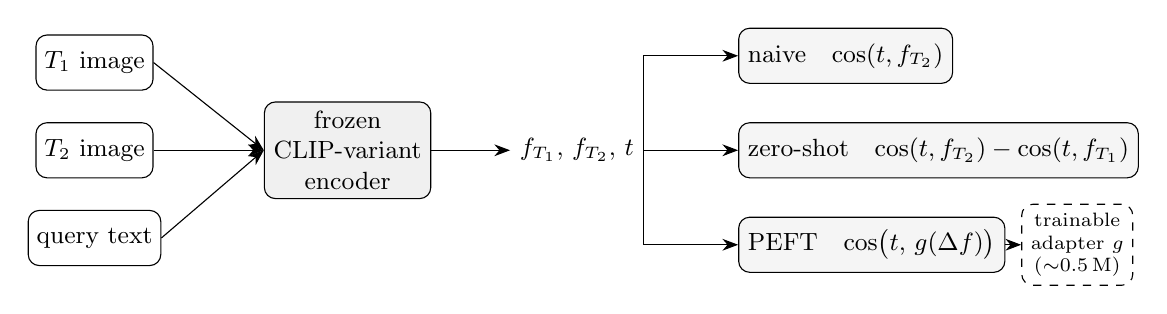
\begin{tikzpicture}[
        font=\small,
        box/.style={draw, rounded corners, minimum height=7mm, align=center, inner sep=3pt},
        enc/.style={draw, fill=black!6, rounded corners, minimum height=9mm, align=center},
        score/.style={draw, rounded corners, fill=black!4, minimum height=7mm, align=center},
        >={Stealth[length=2mm]}, node distance=4mm and 9mm
        ]
        % inputs
        \node[box] (t1) {$T_1$ image};
        \node[box, below=of t1] (t2) {$T_2$ image};
        \node[box, below=of t2] (q) {query text};
        % shared frozen encoder
        \node[enc, right=14mm of t2] (E) {frozen\\CLIP-variant\\encoder};
        \draw[->] (t1.east) -- (E.west);
        \draw[->] (t2.east) -- (E.west);
        \draw[->] (q.east)  -- (E.west);
        % embeddings
        \node[right=10mm of E] (emb) {$f_{T_1},\, f_{T_2},\, t$};
        \draw[->] (E.east) -- (emb.west);
        % three scores
        \node[score, right=12mm of emb, yshift=12mm] (naive) {naive\quad $\cos(t, f_{T_2})$};
        \node[score, right=12mm of emb] (zs) {zero-shot\quad $\cos(t,f_{T_2})-\cos(t,f_{T_1})$};
        \node[score, right=12mm of emb, yshift=-12mm] (peft) {PEFT\quad $\cos\!\big(t,\, g(\Delta f)\big)$};
        \draw[->] (emb.east) |- (naive.west);
        \draw[->] (emb.east) -- (zs.west);
        \draw[->] (emb.east) |- (peft.west);
        % adapter annotation
        \node[draw, dashed, rounded corners, right=2mm of peft, font=\scriptsize, align=center]
            (g) {trainable\\adapter $g$\\($\sim$0.5\,M)};
        \draw[->, dashed] (peft.east) -- (g.west);
    \end{tikzpicture}
    \caption{The three retrieval scores share one frozen CLIP-variant encoder. Only
    the PEFT branch trains a small adapter $g$ over the change feature $\Delta f$ (in
    \texttt{difference} or \texttt{concatenate} mode); the naive and zero-shot scores
    require no training. The naive score ignores $T_1$ entirely (change type), whereas
    the zero-shot $\Delta$-similarity measures how much more present the query becomes
    from $T_1$ to $T_2$ (change transition).}
    \label{fig:scoringmodes}
\end{figure}

\paragraph{Localised patch scoring.}
A global $\Delta$ over two whole-tile embeddings dilutes a change confined to a
small region. The localised scorer therefore embeds each timestep into a grid of
per-patch embeddings (dense features from the frozen encoder's patch tokens,
following the dense-CLIP recipe~\cite{maskclip}) and computes a per-patch
$\Delta$-similarity
$\cos(t, P2_p) - \cos(t, P1_p)$; the pair score \texttt{patch\_top3} is the mean
of the top-3 per-patch deltas (\texttt{scripts/patch\_eval.py}). The same
per-patch $\Delta$-field, conditioned on the query, is the change heatmap shown
in the app and scored against masks in Section~\ref{sec:localization}. Variants
of the aggregation (soft-attention, spatial smoothing, a query-geometry gate) and
a global/patch fusion are evaluated in Section~\ref{sec:ablations}.

\paragraph{LoRA adaptation.}
As an alternative to the projection-head adapter, LoRA~\cite{lora} adapts the
visual encoder's feed-forward projections in place (Section~\ref{sec:ablations}),
keeping the backbone otherwise frozen and adding under 0.5\% of parameters.


\section{Data and encoders}
\label{sec:data}

\paragraph{Dynamic EarthNet (primary).}
DEN is served from the $\sim$7\,GB DynNet preprocessed subset (in preference to
the $\sim$525\,GB raw mirror): per-AOI daily RGB JPEGs ($\approx$730 frames per
AOI) plus \texttt{labels/<AOI>.npy} of shape $(24, 1024, 1024)$ monthly LULC,
with a \texttt{split.json} (55 train / 10 val / 10 test AOIs). The 24 monthly
label maps form the change timeline; each month maps to a representative daily
RGB frame. These preprocessed label maps agree with the official
torchgeo~\cite{torchgeo} Dynamic EarthNet raster masks
(\texttt{torchgeo/dynamic\_earthnet}) to 99.9999\% per-pixel class agreement on
the AOI tiles present in both releases (3 AOIs, 75.5\,M valid pixels),
confirming the preprocessing preserves the published ground truth; the
preprocessed subset additionally retains the held-out test labels the official
release withholds. A deterministic synthetic DEN fixture
(\texttt{scripts/make\_den\_fixture.py}) reproduces the on-disk layout and an
engineered label signal (urban growth, deforestation, seasonal snow-melt, stable
negatives), so the full pipeline is testable in seconds with no network.

DEN also provides an on-disk near-infrared band (\texttt{\_infra.jpeg}, one
grayscale frame per daily timestep), exposed through three colour modes:
\texttt{rgb} (standard 3-channel), \texttt{nrg} (NIR-Red-Green false-colour) and
\texttt{ndvi} (single-band NDVI replicated across three channels). The working
corpus is 605 bimonthly pairs on the train split, and 110 pairs each on val and
test.

\paragraph{QFabric (secondary).}
QFabric~\cite{qfabric} validates the dataset-agnostic design on a different
taxonomy, sensor, and crop scale, using the polygon-centred crops from
\texttt{jirvin16/TEOChatlas}~\cite{teochat} with the real QFabric change-type
labels (the TEOChatlas RQA2 answers; 27{,}879 labelled crops) and, separately,
the RQA5 per-timepoint development-status answers for a temporal transition task.

\paragraph{LEVIR-CC (human change captions).}
LEVIR-CC~\cite{levircc} provides a fundamentally different label source: 10{,}077
bi-temporal building-change pairs ($256\times256$, 0.5\,m), each with five
human-written change captions and a binary change flag (5{,}038 changed /
5{,}039 unchanged). The captions are parsed into open-vocabulary change tags
(building, road, demolition, vegetation, water) so that free-text queries map
directly to caption-grounded relevance (\texttt{src/datasets/levir\_cc.py}),
testing the engine on salient, well-described change in genuine human language
and complementing DEN's subtle spectral transitions and QFabric's categorical
types.

\paragraph{LEVIR-MCI (localisation masks on the LEVIR pairs).}
LEVIR-MCI~\cite{levirmci} is a strict superset of LEVIR-CC - the same 10{,}077
pairs and captions, plus a pixel-level building/road change mask per pair. It is
stored once and serves both \texttt{levir\_cc} and \texttt{levir\_mci}
(\texttt{src/datasets/levir\_mci.py}); the masks make the change-heatmap
deliverable quantitatively measurable (Section~\ref{sec:localization}).

\paragraph{SECOND-CC (open-vocabulary breadth + semantic masks).}
SECOND-CC~\cite{secondcc} pairs 6{,}041 bi-temporal scenes with 30{,}205 human
change captions and six-class SECOND~\cite{second} semantic maps for both
phases (ground, tree, low-vegetation, water, building, playground). It is the
breadth counterpart to LEVIR-CC, whose change is almost entirely building/road:
SECOND-CC's captions span a far wider land-cover vocabulary, and its per-phase
semantic maps give both retrieval relevance (caption tags) and localisation
ground truth (per-class and directed-transition change masks), through the same
protocol (\texttt{src/datasets/second\_cc.py}).

\paragraph{Encoders.}
Table~\ref{tab:encoders} lists the three frozen CLIP-variant encoders. All
embeddings are $L_2$-normalised; the dimension automatically drives cache and
index sizing.

\begin{table}[H]
    \centering
    \caption{The three frozen vision-language encoders.}
    \label{tab:encoders}
    \begin{tabular}{lllr}
        \toprule
        \textbf{Encoder} & \textbf{Backbone} & \textbf{Pre-training} & \textbf{Dim} \\
        \midrule
        \texttt{clip\_vitl14} & ViT-L/14 (HuggingFace CLIP)        & general (CLIP)       & 768 \\
        \texttt{georsclip}    & ViT-B/32 (\texttt{open\_clip})     & RS5M (remote sensing) & 512 \\
        \texttt{remoteclip}   & ViT-L/14 (\texttt{open\_clip})     & RemoteCLIP            & 768 \\
        \bottomrule
    \end{tabular}
\end{table}


\section{Evaluation protocol and metrics}
\label{sec:eval}

Evaluation is label-grounded: a fixed query set is defined per dataset, each
query maps to a relevance rule over the derived \texttt{PairLabel}, and the
ranked corpus is scored with the information-retrieval metrics of
Section~\ref{sec:background}.

\paragraph{Relevance.}
For the captioned and masked datasets (LEVIR-CC, SECOND-CC, QFabric), relevance
is the caption or change-type predicate that a query names. For DEN, relevance is
derived from the per-class \emph{pixel-fraction} change the monthly LULC labels
already encode: a pair is a positive for a change-type query when at least 5\% of
its pixels undergo that class transition. This pixel-fraction rule makes 9 of 10
DEN change-types evaluable (new buildings 14 positives, deforestation 13, soil
25, water 9; only snow is genuinely absent from the subset). A coarser
alternative - counting a pair only when the dominant class of the whole
$1024^2$ tile flips - is satisfied by just 8.6\% of pairs (71/825), 44 of them
wetland$\leftrightarrow$agriculture, and is too sparse to evaluate most queries;
pixel-fraction relevance is therefore the reference rule for DEN, and the two are
contrasted directly in Section~\ref{sec:denmain}.

\paragraph{Metrics.}
We report per-query and macro Recall@$K$, mAP, and a seasonal-drift figure (the
fraction of non-relevant top-$K$ retrievals that involve snow/ice - seasonal
events wrongly returned for permanent-change queries). mAP is macro-averaged only
over queries with at least one positive in the corpus, so the evaluable query set
can differ per split. Two interpretive caveats follow from
Section~\ref{sec:background}: a random ranker scores mAP $\approx$ prevalence
(0.17 on QFabric-TEO, 0.08 on DEN-test), so mAP is read against that floor; and
Recall@$K$ on large relevant sets is ceiling-bounded (with 480 relevant pairs,
$R@10 \le 10/480 = 0.021$), so QFabric is judged by mAP only. Change-heatmap
localisation is scored on the LEVIR-MCI and SECOND-CC masks by the
pointing-game~\cite{pointinggame} metric and patch-AP, each against the encoder's
own random-patch floor.

\paragraph{Cross-validation and significance.}
Because a single 110-pair split is high-variance, the generalisation estimate is
5-fold \emph{leave-one-AOI-out} cross-validation over the merged 75-AOI,
825-pair corpus, partitioning by AOI so no area appears in both train and
evaluation. For learned adapters this leakage control is essential: an adapter
evaluated on areas it trained on measures memorisation, not retrieval.
Significance is assessed against a Monte-Carlo random-ranking baseline (the
relevant set fixed, the ranking shuffled)~\cite{permtest}, with
bootstrap~\cite{bootstrap} confidence intervals and
Benjamini--Hochberg~\cite{benjaminihochberg} FDR correction across the query
set; a query is reported as significant only after FDR correction.


\section{Experiments and results}
\label{sec:results}

All headline experiments use real Dynamic EarthNet. The fast test suite (mock
encoders, synthetic fixture, no network) passes; the full suite additionally runs
the real-CLIP text-encoder test (skipped unless its weights are present) and covers
the embeddings cache and round-trip, retrieval
(naive/zero\_shot/peft), benchmark metrics, PEFT training (loss decreases,
save/load), the encoder protocol/registry, and the app's \texttt{query()} path
(real fixture tiles + heatmap + seasonal note). We report the cross-validated DEN
result first (Section~\ref{sec:denmain}), since it is the generalisation verdict,
then the evidence that learned adapters memorise (Section~\ref{sec:memorisation}),
the ablations that locate the signal (Section~\ref{sec:ablations}), robustness
(Section~\ref{sec:robustness}), and the cross-dataset validation that establishes
the salience law (Section~\ref{sec:crossdataset}).

\subsection{Main result on Dynamic EarthNet}
\label{sec:denmain}

Under the cross-validated protocol of Section~\ref{sec:eval}, the defensible DEN
result is narrow but honest: a frozen, RS-pre-trained encoder (GeoRSCLIP) with
NIR false-colour and localised patch scoring retrieves construction change (new
buildings, urban expansion) and large-area wetland change above chance, with new
water borderline, at $\approx$0.20 cross-validated mAP; no learned adapter beats
it on held-out areas. Table~\ref{tab:cv} traces the GeoRSCLIP+NRG estimate across
the relevance rule and the scoring choice.

\begin{table}[H]
    \centering
    \caption{GeoRSCLIP NRG zero-shot on DEN: single-split mAP is high-variance,
    while the cross-validated estimate is the generalisation verdict. ``S1'' =
    pixel-fraction relevance; ``S3'' = patch-level scoring. Random baseline
    $\approx$ 0.08.}
    \label{tab:cv}
    \begin{tabular}{lccc}
        \toprule
        \textbf{Evaluation} & \textbf{test split} & \textbf{full corpus} & \textbf{5-fold CV} \\
        \midrule
        dominant-flip relevance      & 0.426 & 0.037 & $0.100 \pm 0.139$ \\
        + fraction relevance (S1)    & -   & 0.091 & $0.139 \pm 0.024$ \\
        + patch top-3 scoring (S3)   & -   & 0.122 & $\mathbf{0.193 \pm 0.051}$ \\
        \bottomrule
    \end{tabular}
\end{table}

\paragraph{Single-split variance.}
The widely-quoted 0.426 mAP for GeoRSCLIP+NRG is a single 110-pair test split on
which the cross-validation folds span 0.032--0.348; that split coincides with the
easy high-wetland fold. The 5-fold AOI cross-validated estimate of the same
configuration is $0.100 \pm 0.139$ (full-corpus 0.037), so the single split
overstates generalisation by roughly twofold and only the cross-validated figure
should be read as the result.

\paragraph{Relevance and locality.}
The pixel-fraction relevance rule (Section~\ref{sec:eval}) roughly triples
full-corpus mAP and tightens the cross-validation interval to $0.139 \pm 0.024$
by making nine change-types evaluable rather than three. Beyond relevance, the
remaining ceiling is the global embedding: differencing two whole-tile $1024^2$
embeddings dilutes a small change region, leaving localised change-types (new
buildings, urban expansion, water) near chance. Scoring from per-patch embeddings
with \texttt{patch\_top3} (Section~\ref{sec:methods}) lifts cross-validated mAP to
$0.193 \pm 0.051$ - the best DEN configuration - and makes new buildings
($q{=}0.003$) and urban expansion ($q{=}0.006$) beat random under FDR correction
for the first time, with new water borderline ($q{=}0.053$)
(Figure~\ref{fig:cvprogression}). Diffuse large-area wetland change still prefers
the global score, so the two are complementary. GeoRSCLIP's coarse 49-patch grid
beats CLIP-L/14's finer 256-patch grid (0.193 vs 0.149), so domain pre-training
outweighs patch resolution.

\begin{figure}[H]
    \centering
    
\includegraphics[width=\linewidth]{cv_progression.png}
    \caption{DEN result decomposition (GeoRSCLIP+NRG). Left: the high-variance
    single-split mAP versus the cross-validated estimate, and the effect of
    pixel-fraction relevance (S1) and localised patch scoring (S3), which together
    reach $\approx$0.20 cross-validated mAP. Right: per-query, patch-level scoring
    (S3) recovers localised change-types (buildings/urban/water) that global
    pooling leaves at chance ($*$ = beats random, $p<0.05$).}
    \label{fig:cvprogression}
\end{figure}

\paragraph{The frozen adapter does not help out of distribution.}
Leakage-free cross-validated PEFT on GeoRSCLIP+NRG ($0.196 \pm 0.049$, fraction
relevance) overlaps frozen zero-shot ($0.139 \pm 0.024$) within fold variance -
neither a collapse nor a gain - so low-compute fine-tuning is not shown to
improve retrieval out of distribution. The high in-distribution PEFT figures
(0.42--0.998) are the adapter scored on its own training pairs, as
Section~\ref{sec:memorisation} establishes directly.

\subsection{Learned adapters memorise the training areas}
\label{sec:memorisation}

The in-distribution and cross-split measurements isolate why the adapters do not
generalise. Table~\ref{tab:indist} reports the train split, where the PEFT column
is the adapter evaluated on the very pairs it was trained on, so it measures
memorisation capacity rather than retrieval.

\begin{table}[H]
    \centering
    \caption{Training-set fit (train split, 605 pairs, RGB, \texttt{difference}) -
    PEFT scored on its own training pairs (memorisation), not a held-out result.}
    \label{tab:indist}
    \begin{tabular}{lcccc}
        \toprule
        \textbf{Encoder} & \textbf{naive} & \textbf{zero-shot} & \textbf{PEFT} & \textbf{PEFT R@10} \\
        \midrule
        CLIP ViT-L/14 (768-d)       & 0.031 & 0.043 & \textbf{0.420} & 0.36 \\
        GeoRSCLIP ViT-B/32 (512-d)  & 0.027 & 0.040 & \textbf{0.335} & 0.26 \\
        RemoteCLIP ViT-L/14 (768-d) & 0.024 & 0.057 & \textbf{0.352} & 0.30 \\
        \bottomrule
    \end{tabular}
\end{table}

Three observations follow. First, zero-shot is near chance in-distribution:
$\Delta$-similarity beats the naive image baseline only marginally, because CLIP
and GeoRSCLIP embed scene appearance rather than directional land-cover
transition, so differencing two normalised global embeddings discards the
localised change signal. Second, the $\sim$8--10$\times$ PEFT lift shows the
adapter memorises the 55 training AOIs (the same train fit reaches mAP 0.998 on
QFabric, Section~\ref{sec:qfabricpeft}), not that it retrieves. Third, this
train-fit ranking reverses on held-out data, where GeoRSCLIP leads
(Table~\ref{tab:crosssplit}).

\begin{figure}[H]
    \centering
    \begin{subfigure}{0.49\linewidth}
        \centering
        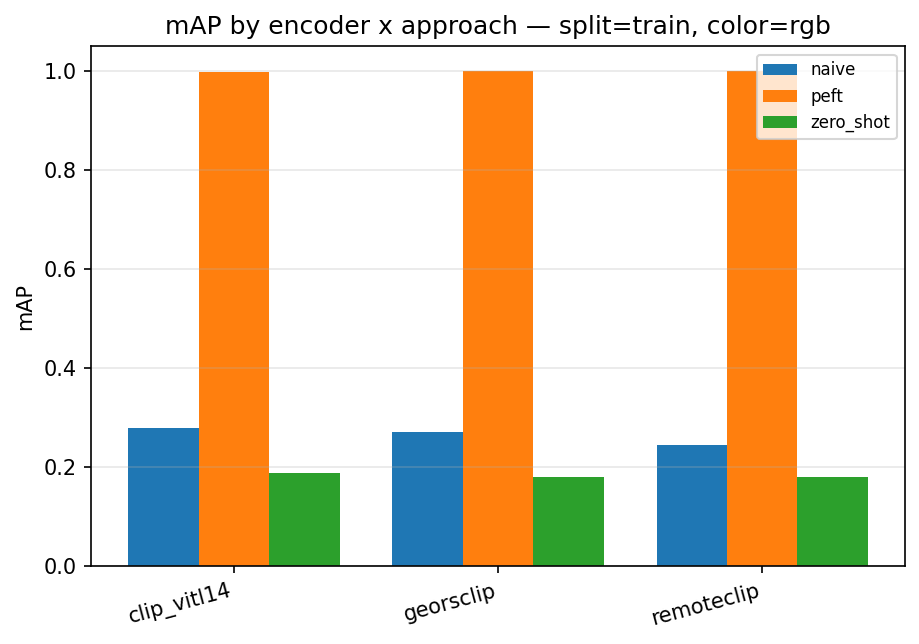
\includegraphics[width=\linewidth]{map_bars__train__rgb.png}
        \caption{train split (in-distribution).}
        \label{fig:mapbars_train}
    \end{subfigure}\hfill
    \begin{subfigure}{0.49\linewidth}
        \centering
        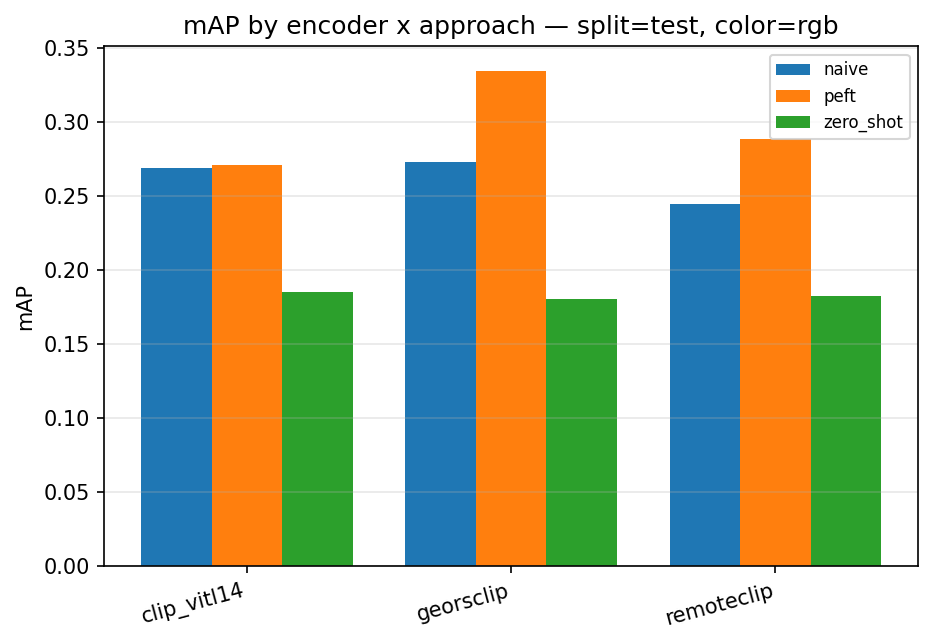
\includegraphics[width=\linewidth]{map_bars__test__rgb.png}
        \caption{held-out test split.}
        \label{fig:mapbars_test}
    \end{subfigure}
    \caption{mAP by encoder $\times$ approach (RGB). The large PEFT bars on train
    (\subref{fig:mapbars_train}) collapse to the frozen scores on the held-out test
    split (\subref{fig:mapbars_test}), where the training-free baselines (GeoRSCLIP
    zero-shot in particular) are competitive - the memorisation signature.}
    \label{fig:mapbars}
\end{figure}

\begin{figure}[H]
    \centering
    \begin{subfigure}{0.49\linewidth}
        \centering
        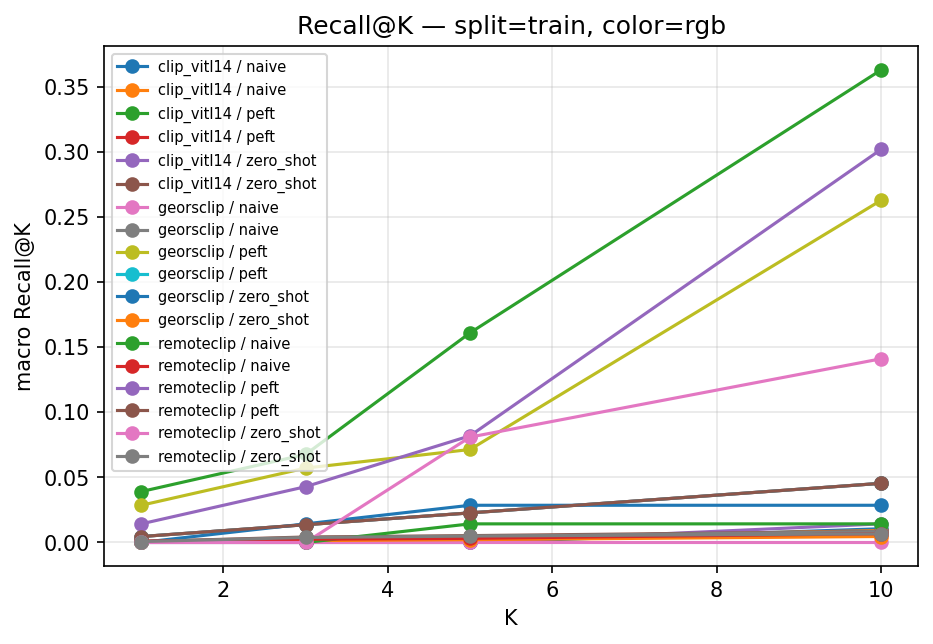
\includegraphics[width=\linewidth]{recall_curves__train__rgb.png}
        \caption{train split.}
        \label{fig:recall_train}
    \end{subfigure}\hfill
    \begin{subfigure}{0.49\linewidth}
        \centering
        
\includegraphics[width=\linewidth]{recall_curves__test__rgb.png}
        \caption{held-out test split.}
        \label{fig:recall_test}
    \end{subfigure}
    \caption{Macro Recall@$K$ versus $K$ for every encoder $\times$ approach (RGB),
    the brief's second retrieval metric alongside mAP. Recall@$K$ is bounded by the
    large relevant-set sizes, so the curves are read for relative ordering, not
    absolute height.}
    \label{fig:recall}
\end{figure}

\begin{figure}[H]
    \centering
    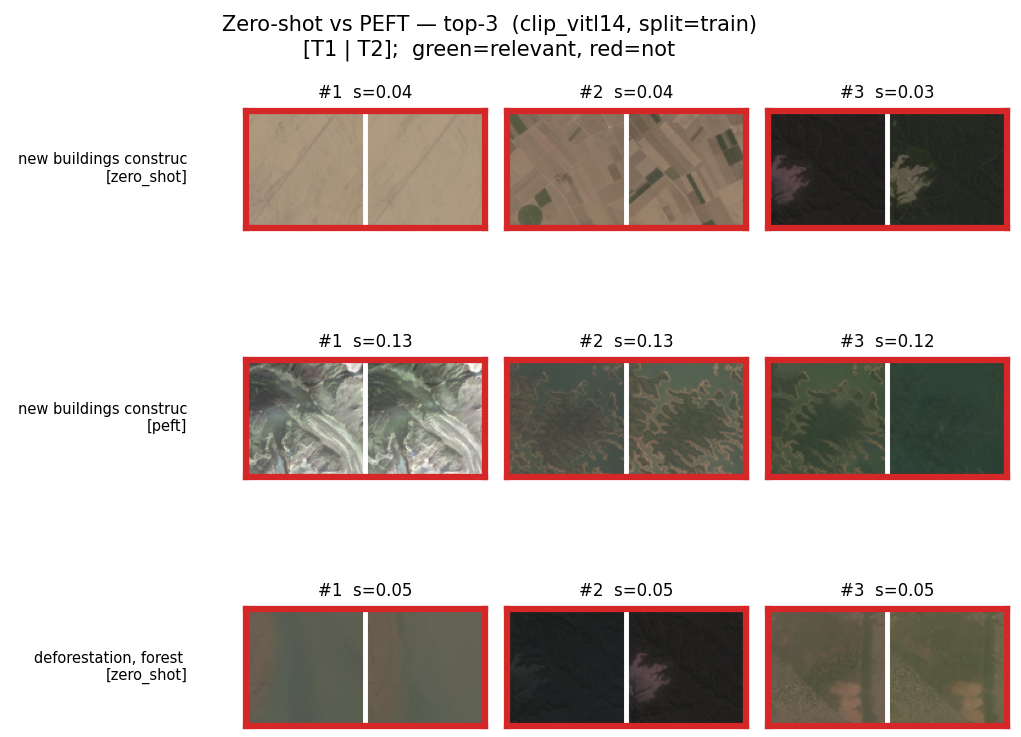
\includegraphics[width=\linewidth]{zeroshot_vs_peft__clip_vitl14__train_part1.png}
    \label{fig:zsvspeft_part1}
\end{figure}

\begin{figure}[H]
    \centering
    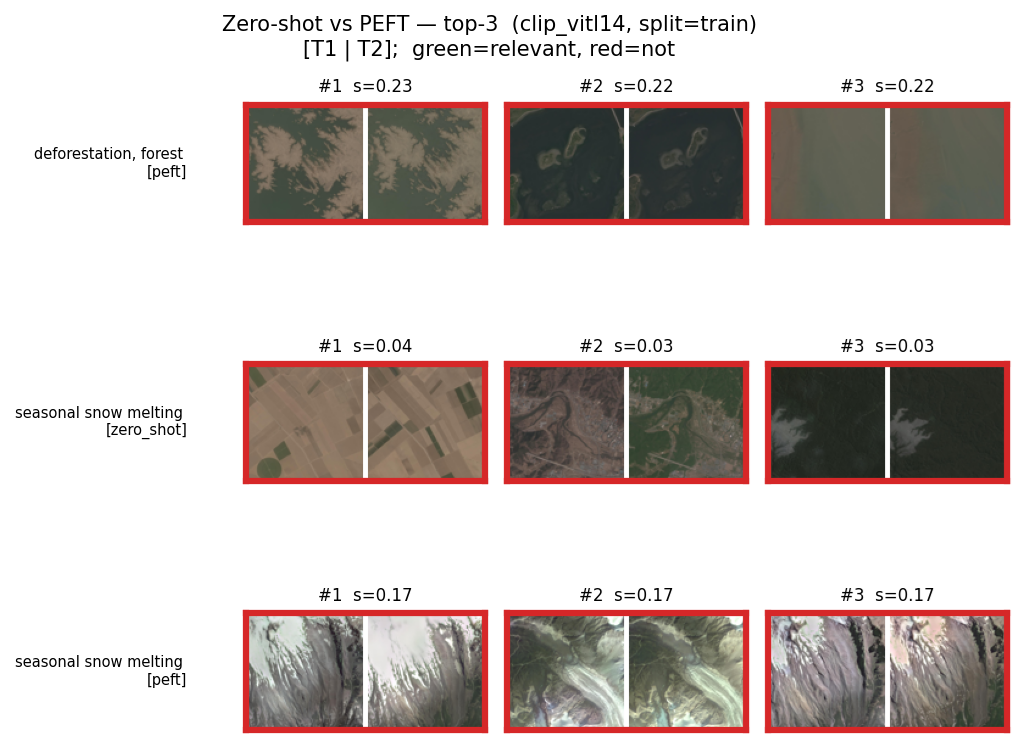
\includegraphics[width=\linewidth]{zeroshot_vs_peft__clip_vitl14__train_part2.png}
    \caption{Qualitative zero-shot vs PEFT (CLIP, train): top-3 retrievals per
    query, $[T_1 \mid T_2]$, green = relevant. The adapter sharpens scores, but
    the gain is concentrated on the classes its weak captions cover.}
    \label{fig:zsvspeft}
\end{figure}

Training the adapter on the train split and evaluating across train/val/test
makes the collapse explicit (Table~\ref{tab:crosssplit}). On unseen val and test
AOIs the adapter is equal to or worse than zero-shot, while GeoRSCLIP zero-shot
reaches 0.299 mAP on the test split with no training at all.

\begin{table}[H]
    \centering
    \caption{Cross-split mAP (adapter trained on train; RGB, \texttt{difference}).}
    \label{tab:crosssplit}
    \begin{tabular}{llccc}
        \toprule
        \textbf{Encoder} & \textbf{approach} & \textbf{train} & \textbf{val} & \textbf{test} \\
        \midrule
        CLIP ViT-L/14       & naive     & 0.031 & 0.053 & 0.046 \\
        CLIP ViT-L/14       & zero-shot & 0.043 & 0.051 & 0.043 \\
        CLIP ViT-L/14       & \textbf{PEFT} & \textbf{0.420} & \textbf{0.042} & \textbf{0.040} \\
        GeoRSCLIP ViT-B/32  & naive     & 0.027 & 0.030 & 0.061 \\
        GeoRSCLIP ViT-B/32  & zero-shot & 0.040 & 0.036 & 0.299 \\
        GeoRSCLIP ViT-B/32  & \textbf{PEFT} & \textbf{0.335} & \textbf{0.087} & \textbf{0.041} \\
        RemoteCLIP ViT-L/14 & naive     & 0.024 & 0.029 & 0.121 \\
        RemoteCLIP ViT-L/14 & zero-shot & 0.057 & 0.025 & 0.050 \\
        RemoteCLIP ViT-L/14 & \textbf{PEFT} & \textbf{0.352} & \textbf{0.028} & \textbf{0.103} \\
        \bottomrule
    \end{tabular}
\end{table}

\subsection{Ablations: what carries the signal}
\label{sec:ablations}

\paragraph{Colour mode.}
Three colour modes are compared (zero-shot mAP, all three splits) in
Table~\ref{tab:nir}. NRG is the best colour mode on held-out test for every
encoder.

\begin{table}[H]
    \centering
    \caption{Colour-mode ablation (zero-shot mAP). NRG is the best colour mode on
    held-out test for every encoder. Best test per encoder in bold.}
    \label{tab:nir}
    \begin{tabular}{llccc}
        \toprule
        \textbf{Encoder} & \textbf{color} & \textbf{train} & \textbf{val} & \textbf{test} \\
        \midrule
        CLIP ViT-L/14 & RGB  & 0.043 & 0.051 & 0.043 \\
        CLIP ViT-L/14 & NRG  & 0.033 & 0.066 & \textbf{0.104} \\
        CLIP ViT-L/14 & NDVI & 0.032 & 0.045 & 0.064 \\
        GeoRSCLIP     & RGB  & 0.040 & 0.036 & 0.299 \\
        GeoRSCLIP     & \textbf{NRG}  & 0.025 & 0.030 & \textbf{0.426} \\
        GeoRSCLIP     & NDVI & 0.028 & 0.065 & 0.216 \\
        RemoteCLIP    & RGB  & 0.057 & 0.025 & 0.050 \\
        RemoteCLIP    & NRG  & 0.023 & 0.047 & \textbf{0.129} \\
        RemoteCLIP    & NDVI & 0.022 & 0.048 & 0.055 \\
        \bottomrule
    \end{tabular}
\end{table}

NRG hurts on train ($-0.010$ to $-0.034$) but substantially helps on test
($+0.061$ CLIP, $+0.127$ GeoRSCLIP, $+0.079$ RemoteCLIP). NDVI usually lands
between NRG and RGB (though for GeoRSCLIP its single-channel collapse drops it
below even RGB on test, 0.216 vs 0.299): NDVI provides some NIR signal but
collapses all spectral texture into a single channel replicated across R/G/B, so
the RS-pretrained encoders cannot exploit the inter-channel colour contrasts that
NRG preserves. RemoteCLIP NRG (test 0.129) improves over RGB (0.050) but lags
GeoRSCLIP NRG, whose RS5M pre-training gives a stronger prior for the NIR-Green
spectral contrast characteristic of vegetation transitions. The single-split NRG
lift for GeoRSCLIP (0.426) is a high-variance fold (cross-validated
$0.100 \pm 0.139$, Section~\ref{sec:denmain}); NRG remaining the best colour mode
for every encoder, and the encoder ordering (GeoRSCLIP $\gg$ CLIP $\approx$
RemoteCLIP), both hold under cross-validation.


\paragraph{Change-feature mode: difference vs concatenate.}
\label{sec:concat}
Re-training the adapter under \texttt{concatenate} (same recipe, RGB, 40 epochs)
and comparing PEFT mAP across splits (Table~\ref{tab:concat}) shows that keeping
both endpoints overfits less.

\begin{table}[H]
    \centering
    \caption{PEFT change-feature mode: difference vs concatenate (RGB).
    Best per encoder/column in bold.}
    \label{tab:concat}
    \begin{tabular}{llccc}
        \toprule
        \textbf{Encoder} & \textbf{mode} & \textbf{train} & \textbf{val} & \textbf{test} \\
        \midrule
        CLIP ViT-L/14 & difference  & \textbf{0.420} & 0.042 & 0.040 \\
        CLIP ViT-L/14 & concatenate & 0.370 & \textbf{0.081} & \textbf{0.050} \\
        GeoRSCLIP     & difference  & \textbf{0.335} & \textbf{0.087} & 0.041 \\
        GeoRSCLIP     & concatenate & 0.275 & 0.086 & \textbf{0.070} \\
        RemoteCLIP    & difference  & 0.352 & 0.028 & \textbf{0.103} \\
        RemoteCLIP    & concatenate & \textbf{0.359} & \textbf{0.109} & 0.078 \\
        \bottomrule
    \end{tabular}
\end{table}

Concatenate consistently lowers in-distribution train mAP (CLIP $-0.050$,
GeoRSCLIP $-0.060$) but raises held-out val for all three encoders and test for
two of three: keeping both endpoints rather than collapsing to their difference
preserves absolute land-cover context the adapter can use to generalise, at the
cost of training-set fit. The effect is modest and PEFT still does not beat
frozen zero-shot out of distribution, but \texttt{concatenate} is the
better-generalising change feature.

\paragraph{LoRA on the visual encoder.}
LoRA~\cite{lora} applied to GeoRSCLIP's ViT-B/32 visual encoder targets the FFN
projections \texttt{c\_fc} and \texttt{c\_proj} in each ResBlock: 368{,}640
trainable params out of 88M (0.42\%). The attention output projection
\texttt{out\_proj} is deliberately not adapted - open\_clip's attention is an
\texttt{nn.\allowbreak{}MultiheadAttention} whose forward reads \texttt{out\_proj.weight}
directly (via \texttt{F.\allowbreak{}multi\_\allowbreak{}head\_\allowbreak{}attention\_\allowbreak{}forward}) and never calls
\texttt{out\_proj.forward}, so a LoRA wrapper there receives no gradient.
Training is online (images loaded on the fly) using the same masked symmetric
InfoNCE loss as the ProjectionHead. Table~\ref{tab:lora} compares frozen
zero-shot against LoRA-adapted zero-shot (GeoRSCLIP + NRG, rank=4, $\alpha$=8, 20
epochs).

\begin{table}[H]
    \centering
    \caption{LoRA (GeoRSCLIP + NRG) vs frozen zero-shot. LoRA fits train and
    matches val but collapses on the held-out test split. Best per row in bold.}
    \label{tab:lora}
    \begin{tabular}{lcc}
        \toprule
        \textbf{split} & \textbf{zero\_shot (frozen)} & \textbf{LoRA zero\_shot} \\
        \midrule
        train & 0.025 & \textbf{0.153} \\
        val   & 0.030 & \textbf{0.034} \\
        test  & \textbf{0.426} & 0.071 \\
        \bottomrule
    \end{tabular}
\end{table}

LoRA fits the train split ($0.025 \rightarrow 0.153$) but collapses out of
distribution ($0.071$ on test). That test $0.071$ is numerically just above
ProjectionHead PEFT's RGB test ($0.041$), but the comparison is cross-colour-mode
and both sit at or below the DEN-test random floor ($\approx 0.083$) - neither
learned adapter beats chance on held-out AOIs. A rank/epoch sweep
(Table~\ref{tab:lorasweep}; \texttt{scripts/lora\_sweep.py}, in-memory) finds no
capacity sweet spot.

\begin{table}[H]
    \centering
    \caption{LoRA rank/epoch sweep (GeoRSCLIP + NRG, zero\_shot mAP). Every
    configuration fits train yet collapses on test - no capacity sweet spot.}
    \label{tab:lorasweep}
    \begin{tabular}{ccccc}
        \toprule
        \textbf{rank} & \textbf{$\alpha$} & \textbf{epochs} & \textbf{train} & \textbf{test} \\
        \midrule
        4  & 8  & 20 & 0.153 & 0.071 \\
        8  & 16 & 20 & 0.168 & 0.070 \\
        16 & 32 & 20 & 0.135 & 0.058 \\
        8  & 16 & 40 & 0.146 & 0.059 \\
        \bottomrule
    \end{tabular}
\end{table}

Every rank/epoch setting fits the train split (0.13--0.17, well above the frozen
0.025) yet overfits to test 0.06--0.07; more rank or more epochs only memorise
harder. This reinforces the project's core finding that spectral physics (NRG
false-colour) generalises while learned visual priors only memorise.


\paragraph{Aggregation refinements (honest negatives).}
Several cheaper in-scope refinements were tested and none improved on
\texttt{patch\_top3}, reported here as honest negatives. Averaging the query
embedding over a prompt ensemble is a wash (0.142 cross-validated mAP); fusing
the global $\Delta$-cosine with the patch score by z-scoring and summing hurts
(0.165), the mostly-noise global signal diluting the stronger patch signal; and
two training-free change-attention variants - query-conditioned soft-attention
over the per-patch $\Delta$ (0.137) and $3\times3$ spatial smoothing of the
$\Delta$-map (0.168) - refine the aggregation without breaking the
$\approx$0.20 ceiling. Routing each query by its a-priori spatial geometry -
diffuse phrasings to the global score, localised ones to patch top-3 - scores
$0.186 \pm 0.051$ under the same cross-validation, statistically
indistinguishable from ungated patch top-3 and recovering the same four
FDR-significant queries, so query geometry is not a usable routing signal at this
encoder scale. A learned query-to-patch attention head is deliberately not
pursued, since every trained head on this data memorises the training AOIs with
no held-out gain (Section~\ref{sec:memorisation}).

\subsection{Robustness: seasonal vs permanent}
\label{sec:robustness}

The benchmark reports seasonal drift@$K$ (non-relevant top-$K$ retrievals that
involve snow/ice, for permanent-change queries). On the DEN train split this is
0.00 at all $K$ for every encoder/approach - there is essentially no seasonal
(snow/ice) class in this subset, so seasonal$\rightarrow$permanent confusion does
not arise here. The mechanism is nonetheless implemented and exercised on the
synthetic fixture, which contains a seasonal snow-melt pair: the app flags it
(``involves snow/ice - likely SEASONAL, not permanent'') and the benchmark
counts it as drift if mis-retrieved.

The dominant real error is not seasonal confusion but low recall from class
imbalance and weak label-derived captions (many near-stable bimonthly pairs;
agri$\leftrightarrow$wetland visually subtle). The per-query confusion analysis
(\texttt{src/error\_analysis.py}) makes this concrete: on the best test
configuration (GeoRSCLIP + NRG), the wetland queries' top-10 are dominated by
\texttt{stable} pairs (6--7 of 10), so the failure mode is surfacing no-change
pairs (Figure~\ref{fig:confusion}).

\begin{figure}[H]
    \centering
    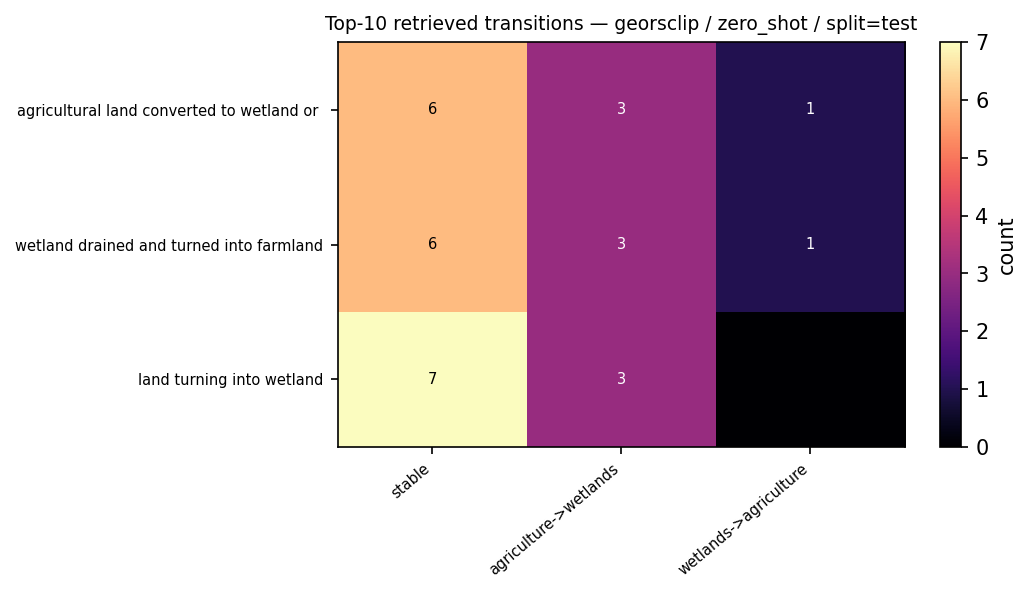
\includegraphics[width=0.8\linewidth]{confusion__georsclip__test__zero_shot.png}
    \caption{Per-query confusion (GeoRSCLIP + NRG zero-shot, test): top-$K$
    retrievals binned by actual label transition; wetland queries are dominated
    by \texttt{stable} pairs.}
    \label{fig:confusion}
\end{figure}

\begin{figure}[H]
    \centering
    \begin{subfigure}{0.49\linewidth}
        \centering
        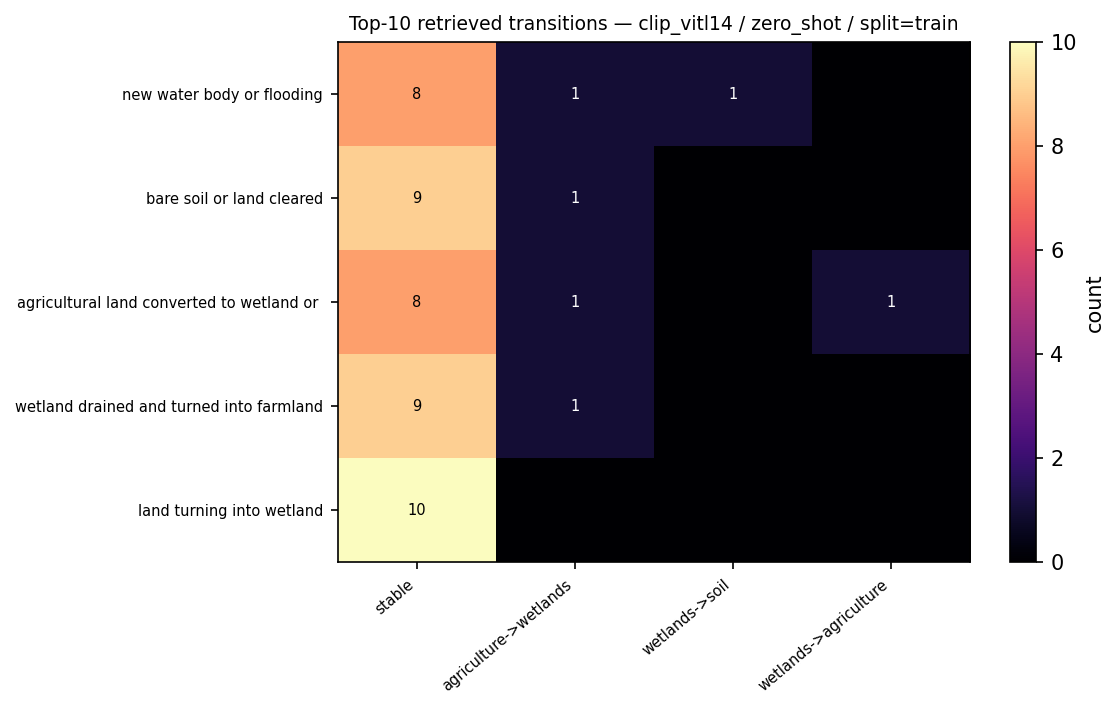
\includegraphics[width=\linewidth]{confusion__clip_vitl14__train__zero_shot.png}
        \caption{zero-shot.}
        \label{fig:confusion_train_zs}
    \end{subfigure}\hfill
    \begin{subfigure}{0.49\linewidth}
        \centering
        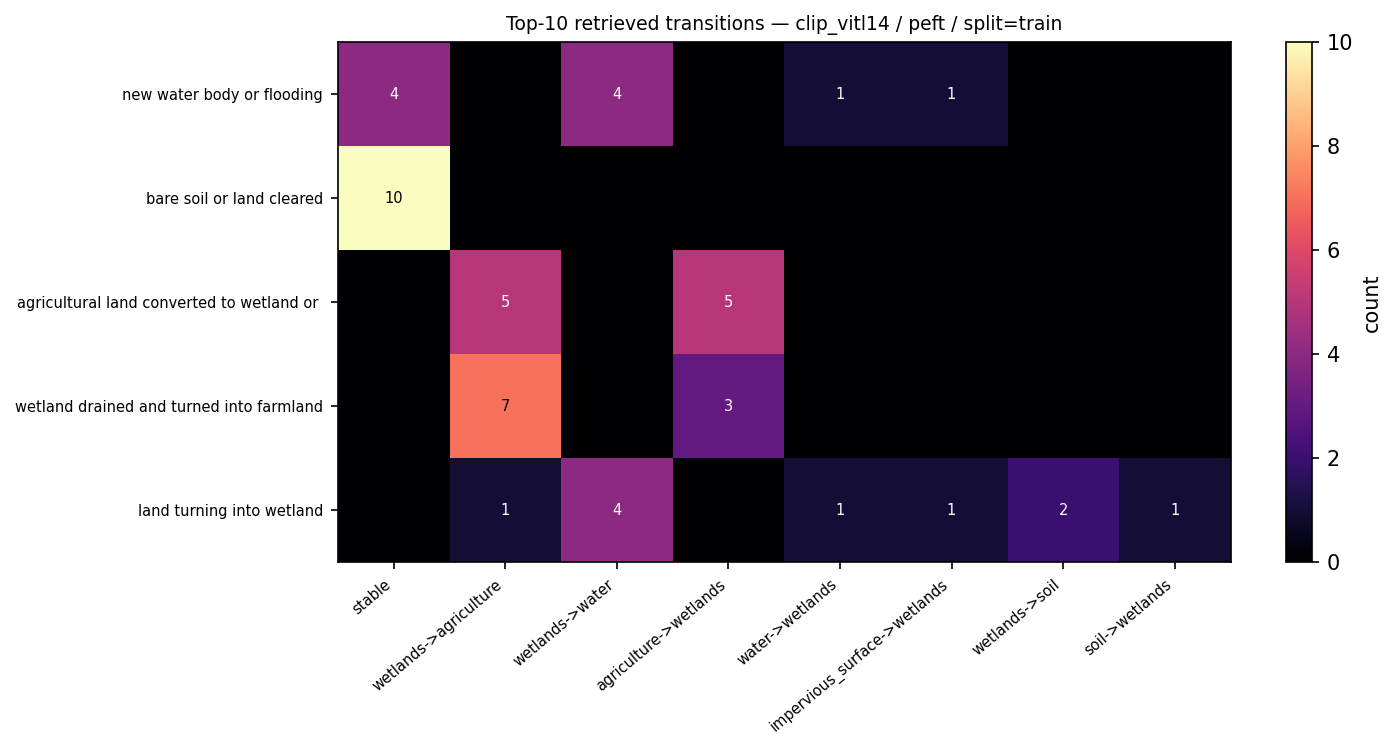
\includegraphics[width=\linewidth]{confusion__clip_vitl14__train__peft.png}
        \caption{PEFT.}
        \label{fig:confusion_train_peft}
    \end{subfigure}
    \caption{In-distribution confusion (CLIP ViT-L/14, train split): top-$K$
    retrievals binned by actual transition. The PEFT adapter
    (\subref{fig:confusion_train_peft}) concentrates each query's retrievals on
    its own positive transition far more sharply than zero-shot
    (\subref{fig:confusion_train_zs}) - the visible face of the train-set
    memorisation of Section~\ref{sec:memorisation}.}
    \label{fig:confusion_train}
\end{figure}

Seasonal robustness is also probed directly. The zero-shot score is turned into a
whole-image binary gate: for a change query $t$ and a pair's $L_2$-normalised
global embeddings, the gate fires when
$\Delta = \cos(t, f_{T_2}) - \cos(t, f_{T_1}) > \tau$. On a stable pair
$f_{T_1} \approx f_{T_2}$, so $\Delta \approx 0$ for any query and every firing is
a false positive; sweeping $\tau$ over the stable subset (DEN's own
\texttt{PairLabel.stable} flag) yields a false-positive-rate curve
(\texttt{src/seasonal\_gate.py}). Table~\ref{tab:seasonalgate} reports the curve
for the strongest configuration (GeoRSCLIP, RGB, test split, 24 stable pairs).

\begin{table}[H]
    \centering
    \caption{Stable-pair false-positive rate of the $\Delta$-similarity gate
    (GeoRSCLIP, RGB, test split; 24 stable pairs, mean stable $\Delta = 0.0125$).}
    \label{tab:seasonalgate}
    \begin{tabular}{ccccc}
        \toprule
        \textbf{mean stable $\Delta$} & \textbf{FPR@0.00} & \textbf{FPR@0.02} & \textbf{FPR@0.05} & \textbf{FPR@0.10} \\
        \midrule
        0.0125 & 0.875 & 0.333 & 0.000 & 0.000 \\
        \bottomrule
    \end{tabular}
\end{table}

Stable pairs carry a near-zero mean $\Delta$-similarity (0.0125), so the
false-positive rate falls to zero once the threshold clears the noise floor, and
is already zero at $\tau = 0.05$. The high 0.875 rate at $\tau = 0$ merely
reflects that any nonzero $\Delta$ trips a zero threshold and is not a failure
mode. The gate confirms that seasonal and illumination drift on stable pairs does
not masquerade as change once a modest threshold is applied.

\subsection{Cross-dataset validation and the salience law}
\label{sec:crossdataset}

The three further datasets test the dataset-agnostic design and the salience
hypothesis of Section~\ref{sec:intro}. QFabric establishes that task geometry
sets the naive-versus-$\Delta$ trade-off; LEVIR-CC and SECOND-CC establish that
recovery scales with change salience; the masks quantify that localisation is
harder than retrieval.

\paragraph{QFabric change-type retrieval.}
Images are the polygon-centred crops from \texttt{jirvin16/TEOChatlas}; labels are
the real QFabric change types (the RQA2 answers), joined to crops by the shared
filename scheme. On a stratified $\leq$120 crops/class subset ($N = 2476$ pairs)
with six change-type queries and frozen encoders (RGB),
Table~\ref{tab:qfabric} reports mAP.

\begin{table}[H]
    \centering
    \caption{QFabric change-type retrieval (frozen encoders, RGB, mAP). naive
    beats zero-shot - the opposite of DEN. Best per row in bold.}
    \label{tab:qfabric}
    \begin{tabular}{lcc}
        \toprule
        \textbf{Encoder} & \textbf{naive} & \textbf{zero-shot} \\
        \midrule
        CLIP ViT-L/14 & \textbf{0.274} & 0.187 \\
        GeoRSCLIP     & \textbf{0.269} & 0.182 \\
        RemoteCLIP    & \textbf{0.233} & 0.180 \\
        \bottomrule
    \end{tabular}
\end{table}

Naive beats zero-shot here, the opposite of DEN. QFabric change types (residential
/ road / industrial \dots) are identifiable from the after-image content alone, so
$\cos(t, f_{T_2})$ wins; the directional $\Delta$-similarity that helped on DEN
here adds noise. The random-ranking baseline is the macro class prevalence, 0.167;
\texttt{naive} (0.274) sits $+0.11$ above chance while \texttt{zero\_shot} (0.187)
is only $+0.02$. Per-query (CLIP naive), the signal concentrates in road (AP
0.50), residential (0.36) and industrial (0.30); demolition (0.25) and commercial
(0.22) are weak; mega\_projects (0.03) is at chance. The pipeline runs end-to-end
on a different taxonomy, sensor, and crop scale with no code changes beyond a
loader and a query set, confirming the dataset-agnostic abstraction and surfacing
a regime in which after-image content outweighs the temporal $\Delta$.


\paragraph{QFabric PEFT.}
\label{sec:qfabricpeft}
Closing the zero-shot-vs-PEFT comparison on QFabric uses a stratified,
crop-disjoint train/test split (train $\leq$120 crops/class, $N$=2422 pairs;
held-out test $N$=2048), a ProjectionHead adapter trained on the train split with
captions phrased like the queries (\texttt{difference}, 40 epochs), evaluated on
both splits (Table~\ref{tab:qfabricpeft}).

\begin{table}[H]
    \centering
    \caption{QFabric PEFT (mAP). Adapter overfits train ($\approx$0.999) but on
    test sits at-or-above naive. Best per row in bold.}
    \label{tab:qfabricpeft}
    \begin{tabular}{llccc}
        \toprule
        \textbf{Encoder} & \textbf{split} & \textbf{naive} & \textbf{zero-shot} & \textbf{PEFT} \\
        \midrule
        CLIP ViT-L/14 & train & 0.278 & 0.189 & \textbf{0.998} \\
        CLIP ViT-L/14 & test  & 0.269 & 0.185 & 0.271 \\
        GeoRSCLIP     & train & 0.271 & 0.180 & \textbf{0.999} \\
        GeoRSCLIP     & test  & 0.272 & 0.181 & \textbf{0.334} \\
        RemoteCLIP    & train & 0.244 & 0.179 & \textbf{0.999} \\
        RemoteCLIP    & test  & 0.245 & 0.183 & \textbf{0.288} \\
        \bottomrule
    \end{tabular}
\end{table}

PEFT overfits train on both datasets ($\approx$0.999 here) but generalises
differently. On held-out QFabric test the adapter is at-or-above \texttt{naive}:
GeoRSCLIP $+0.062$ (0.334, the best QFabric result), RemoteCLIP $+0.043$ (0.288),
CLIP neutral. This contrasts with DEN (Section~\ref{sec:memorisation}), where PEFT
test collapsed below zero-shot (GeoRSCLIP RGB: $0.299 \rightarrow 0.041$). The
difference is what the adapter must learn: QFabric change types are consistent
visual categories (a road looks like a road across crops), so the head learns
transferable features; DEN's directional spectral transitions are subtle and
AOI-specific, so the head memorises training-AOI statistics. PEFT's value is
therefore dataset-dependent: harmful on DEN, mildly helpful on QFabric. Both
effects are small in absolute terms, since a random ranker already scores mAP
$\approx$0.17 on QFabric.


\paragraph{QFabric status-transition retrieval: the regime inverts.}
QFabric also carries a temporal task through the TEOChatlas RQA5/RTQA5 answers:
the per-timepoint development status of each region, on a nine-stage scale from
greenland through land-cleared and construction-started to operational. Joining
each answer to its frame (\texttt{scripts/build\_qfabric\_status\_labels.py},
dataset \texttt{qfabric\_status}) gives every pair a status transition, and six
transition queries (for example ``new building construction has started'') are
relevant only to pairs whose status actually changes; stable pairs become hard
negatives with the same end-state. On a stratified subset of $\leq$120 crops per
final status ($N = 4200$ pairs, frozen encoders, RGB),
Table~\ref{tab:qfabricstatus} reports mAP.

\begin{table}[H]
    \centering
    \caption{QFabric status-transition retrieval (RQA5; frozen, RGB, mAP). The
    directional zero-shot score now matches or beats naive on every encoder,
    inverting the change-type regime of Table~\ref{tab:qfabric}. Best per row in bold.}
    \label{tab:qfabricstatus}
    \begin{tabular}{lcc}
        \toprule
        \textbf{Encoder} & \textbf{naive} & \textbf{zero-shot} \\
        \midrule
        CLIP ViT-L/14 & 0.057 & \textbf{0.057} \\
        GeoRSCLIP     & 0.079 & \textbf{0.084} \\
        RemoteCLIP    & 0.064 & \textbf{0.072} \\
        \bottomrule
    \end{tabular}
\end{table}

The regime inverts: zero-shot is at least as good as naive on all three encoders
($+0.000$ CLIP, $+0.005$ GeoRSCLIP, $+0.007$ RemoteCLIP), the opposite of the
change-type result, where naive led by about 0.09. The directional $\Delta$ is the
appropriate tool for transitions, while after-image content is the appropriate
tool for types - one dataset, two tasks, two regimes. The edge is consistent but
small, and both scores sit just above the 0.043 macro-prevalence baseline:
status-transition retrieval is genuinely hard zero-shot, with long irregular
temporal baselines and many subtle or rare transitions. The signal concentrates in
the visually distinct, well-populated transitions - land cleared (AP 0.17) and
construction started (0.18) - and collapses on the rare or long-range ones
(demolition 0.01, $n=32$; vacant-to-finished building 0.02, $n=64$). Relabelling
the same crops along a temporal axis rather than a categorical one inverts which
scoring approach wins, direct evidence that the naive-versus-$\Delta$ trade-off is
set by task geometry rather than by the dataset.


\paragraph{LEVIR-CC: salience-scaled retrieval.}
LEVIR-CC pairs are parsed into five open-vocabulary change tags from their
captions - building, road, demolition, vegetation, water - and one free-text
query maps to each. On the held-out test split (1929 pairs, frozen encoders,
RGB), Table~\ref{tab:levircc} reports per-query average precision and the
five-query macro. The macro random-ranking baseline is the mean query prevalence,
0.255 (building 45.2\%, road 42.7\%, demolition 14.8\%, vegetation 23.9\%, water
1.0\%).

\begin{table}[H]
    \centering
    \caption{LEVIR-CC open-vocabulary change retrieval (test split, 1929 pairs,
    frozen, RGB; zero-shot average precision per query, with the five-query macro
    mAP). Test positives per query in parentheses. Best per row in bold.}
    \label{tab:levircc}
    \begin{tabular}{lccc}
        \toprule
        \textbf{Query (positives)} & \textbf{GeoRSCLIP} & \textbf{CLIP ViT-L/14} & \textbf{RemoteCLIP} \\
        \midrule
        new buildings or houses (871) & 0.804 & 0.725 & \textbf{0.830} \\
        a new road or street (824)    & 0.571 & 0.631 & \textbf{0.654} \\
        buildings demolished (286)    & \textbf{0.297} & 0.138 & 0.234 \\
        trees or vegetation (462)     & 0.159 & 0.182 & \textbf{0.186} \\
        a lake, pond, or water (19)   & 0.151 & \textbf{0.221} & 0.096 \\
        \midrule
        \textbf{macro mAP (5 queries)} & 0.396 & 0.379 & \textbf{0.400} \\
        \bottomrule
    \end{tabular}
\end{table}

The five-query macro (0.38--0.40 zero-shot; naive 0.41--0.43) is held up by two
strong queries and dragged by three weak ones, so the per-query reading is the
honest one. Building and road change - large, high-contrast, and described in
the vocabulary the CLIP text tower was trained on - are retrieved strongly
(buildings $\approx$0.8, roads $\approx$0.6), whereas demolition, vegetation, and
the 19-positive water class sit at or only just above their prevalence floors.
This is the salience-proportional pattern the project finds in every dataset,
pooled and quantified in Figure~\ref{fig:saliencelaw}. The RS-pre-trained encoders
still gain from the directional $\Delta$ on the strong queries, the same
type-versus-transition split seen on QFabric.

\begin{figure}[H]
    \centering
    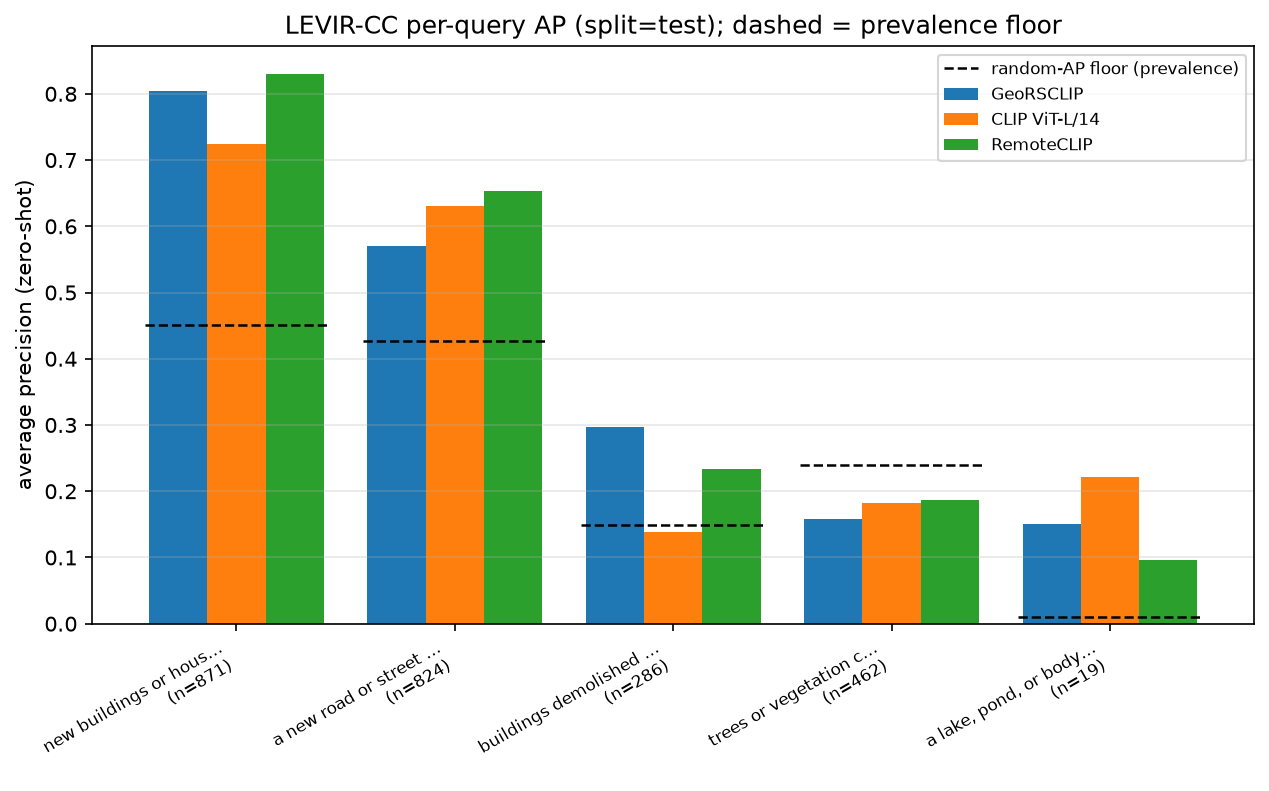
\includegraphics[width=0.95\linewidth]{per_query_ap__levir_cc__test.png}
    \caption{LEVIR-CC per-query zero-shot AP by encoder (test split, RGB), with
    each query's prevalence floor (dashed). Salient building and road change clears
    the floor by a wide margin; demolition, vegetation, and the 19-positive water
    class sit at or only just above it.}
    \label{fig:levircc_ap}
\end{figure}

\paragraph{SECOND-CC: open-vocabulary breadth.}
SECOND-CC~\cite{secondcc} is the breadth counterpart: 6{,}041 pairs with human
captions and six-class semantic maps for both phases. Seven free-text queries
cover the six SECOND classes plus road. Test split, 1{,}227 pairs, frozen
encoders, RGB; macro random-ranking floor 0.297.

\begin{table}[H]
    \centering
    \caption{SECOND-CC zero-shot per-query AP (test split). Buildings dominate;
    every type clears its prevalence floor but only modestly.}
    \label{tab:secondcc}
    \begin{tabular}{lccc}
        \toprule
        \textbf{Query (positives)} & \textbf{GeoRSCLIP} & \textbf{CLIP ViT-L/14} & \textbf{RemoteCLIP} \\
        \midrule
        new buildings/structures (809) & 0.698 & 0.652 & \textbf{0.702} \\
        a new road or street (460)     & \textbf{0.418} & 0.377 & 0.372 \\
        bare ground or land cleared (401) & 0.355 & \textbf{0.372} & 0.362 \\
        trees appeared/cleared (370)   & \textbf{0.341} & 0.313 & 0.334 \\
        low vegetation/grassland (311) & 0.275 & \textbf{0.280} & 0.273 \\
        a water body (167)             & \textbf{0.168} & 0.152 & 0.159 \\
        a playground/sports field (33) & 0.085 & 0.035 & \textbf{0.164} \\
        \midrule
        \textbf{macro mAP (zero-shot)} & 0.334 & 0.312 & \textbf{0.338} \\
        \textbf{macro mAP (naive)}     & \textbf{0.453} & 0.430 & 0.441 \\
        \bottomrule
    \end{tabular}
\end{table}

Across seven change types every query clears its prevalence floor - broader
recovery than DEN, where most queries sat at random - but only modestly: the
zero-shot macro ($\approx$0.33) is $\approx$+0.04 over the 0.297 floor, buildings
($\approx$0.70) dominate, and water/playground are weak. As on QFabric, naive
$>$ zero-shot (macro 0.45 vs 0.33): end-state appearance carries more of these
land-cover categories than the temporal $\Delta$. SECOND-CC thus extends the
project's central law to a wide open vocabulary: recovery scales with the visual
salience and prevalence of the change type, and is weak in absolute terms with
frozen CLIP-variant encoders.

\begin{figure}[H]
    \centering
    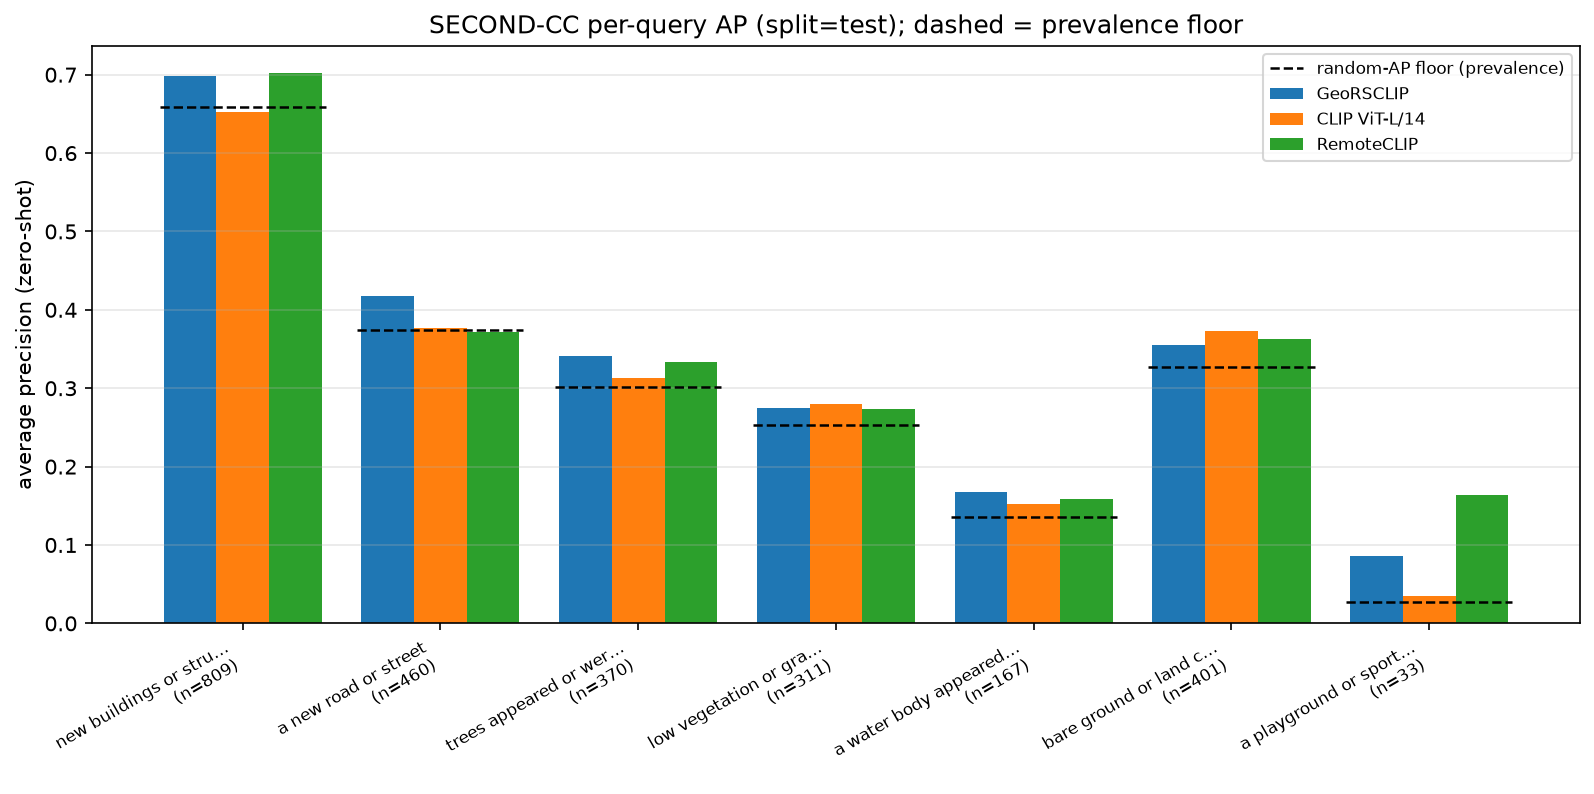
\includegraphics[width=0.95\linewidth]{per_query_ap__second_cc__test.png}
    \caption{SECOND-CC per-query zero-shot AP by encoder (test split, RGB), with
    each query's prevalence floor (dashed). Across all seven change types every
    query clears its floor - broader recovery than DEN - but only modestly,
    with buildings dominating and water/playground weakest.}
    \label{fig:secondcc_ap}
\end{figure}

\paragraph{Quantitative change localisation.}
\label{sec:localization}
The change heatmap is scored on the LEVIR-MCI and SECOND-CC pixel masks. For each
masked query the query-conditioned heatmap (per-patch $\Delta$-similarity
$\cos(t,P2_p)-\cos(t,P1_p)$, the same signal as the patch scorer of
Section~\ref{sec:methods}) is scored by pointing-game~\cite{pointinggame} (is the
highest-$\Delta$ patch a true change patch?) and patch-AP, over pairs that
contain the change with at least one positive patch at grid resolution. Each
encoder is compared only to its own random-patch floor, since the patch grid
differs by encoder (GeoRSCLIP $7\times7$, the ViT-L encoders $16\times16$).

\begin{table}[H]
    \centering
    \caption{LEVIR-MCI change localisation (test split; pointing-game and patch-AP
    against each encoder's random-patch floor). Lift is pointing minus floor.}
    \label{tab:localization}
    \begin{tabular}{llccc}
        \toprule
        \textbf{Encoder (grid)} & \textbf{Class} & \textbf{pointing} & \textbf{floor} & \textbf{lift} \\
        \midrule
        GeoRSCLIP ($7\times7$)     & road     & 0.416 & 0.334 & \textbf{+0.082} \\
        GeoRSCLIP ($7\times7$)     & building & 0.351 & 0.378 & $-0.027$ \\
        RemoteCLIP ($16\times16$)  & road     & 0.312 & 0.208 & \textbf{+0.104} \\
        RemoteCLIP ($16\times16$)  & building & 0.257 & 0.238 & +0.019 \\
        CLIP ViT-L/14 ($16\times16$) & road     & 0.151 & 0.208 & $-0.057$ \\
        CLIP ViT-L/14 ($16\times16$) & building & 0.101 & 0.238 & $-0.137$ \\
        \bottomrule
    \end{tabular}
\end{table}

The heatmap is a weak localiser. Only road change is localised above chance, and
only by the RS-pre-trained encoders (RemoteCLIP $+0.10$, GeoRSCLIP $+0.08$
pointing-game lift); building change is not localised above its floor by any
encoder, and generic CLIP ViT-L \emph{anti-localises} ($-0.14$ on building). On
the SECOND-CC semantic masks the verdict matches - every reliably-sampled class
sits within $\pm$0.04 of its random-patch floor (the lone large value, playground
$+0.30$ on GeoRSCLIP, rests on 22 pairs and does not replicate). This is the
spatial counterpart of the retrieval result: frozen CLIP-variant embeddings
recover change weakly, and localising it - a harder task than retrieving it -
is weaker still, with only RS pre-training buying a modest road signal. The
overlay stays useful for a human in the loop, but it is not a quantitatively
reliable detector.

\paragraph{The salience law.}
Pooled across the open-vocabulary datasets (Figure~\ref{fig:saliencelaw}), the
recovered signal tracks change salience: weak on DEN's subtle spectral
transitions, dataset-dependent on QFabric, strong on LEVIR-CC's salient
building/road change (per-query AP $\approx$0.6--0.8) yet near-random on its
subtle vegetation and sparse water, and above every SECOND-CC prevalence floor
but only modestly. This echoes --- by analogy rather than shared mechanism ---
the classical visual-saliency observation~\cite{saliency} that salient stimuli
dominate perception: here the driver is text--image embedding alignment, not
bottom-up attention, yet salience is the single empirical regularity the project
finds in every dataset.

\begin{figure}[H]
    \centering
    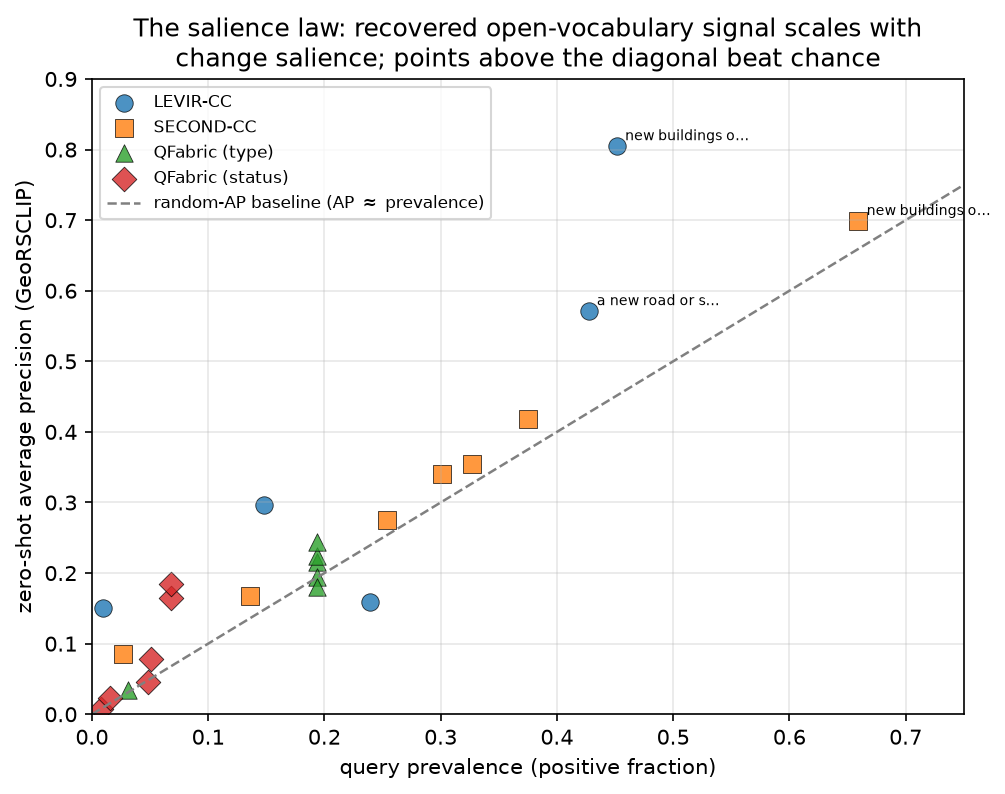
\includegraphics[width=0.82\linewidth]{salience_law__summary.png}
    \caption{The salience law, pooled across the open-vocabulary datasets: each
    point is a per-query zero-shot AP (GeoRSCLIP) against that query's prevalence,
    where a random ranker scores $\text{AP}\approx\text{prevalence}$ (dashed
    diagonal). Salient, well-described construction change (new buildings, roads)
    sits far above chance; subtle, sparse, or rare transitions (water, vegetation,
    status changes) collapse onto the diagonal - the single law this project
    finds in every dataset.}
    \label{fig:saliencelaw}
\end{figure}

\begin{figure}[H]
    \centering
    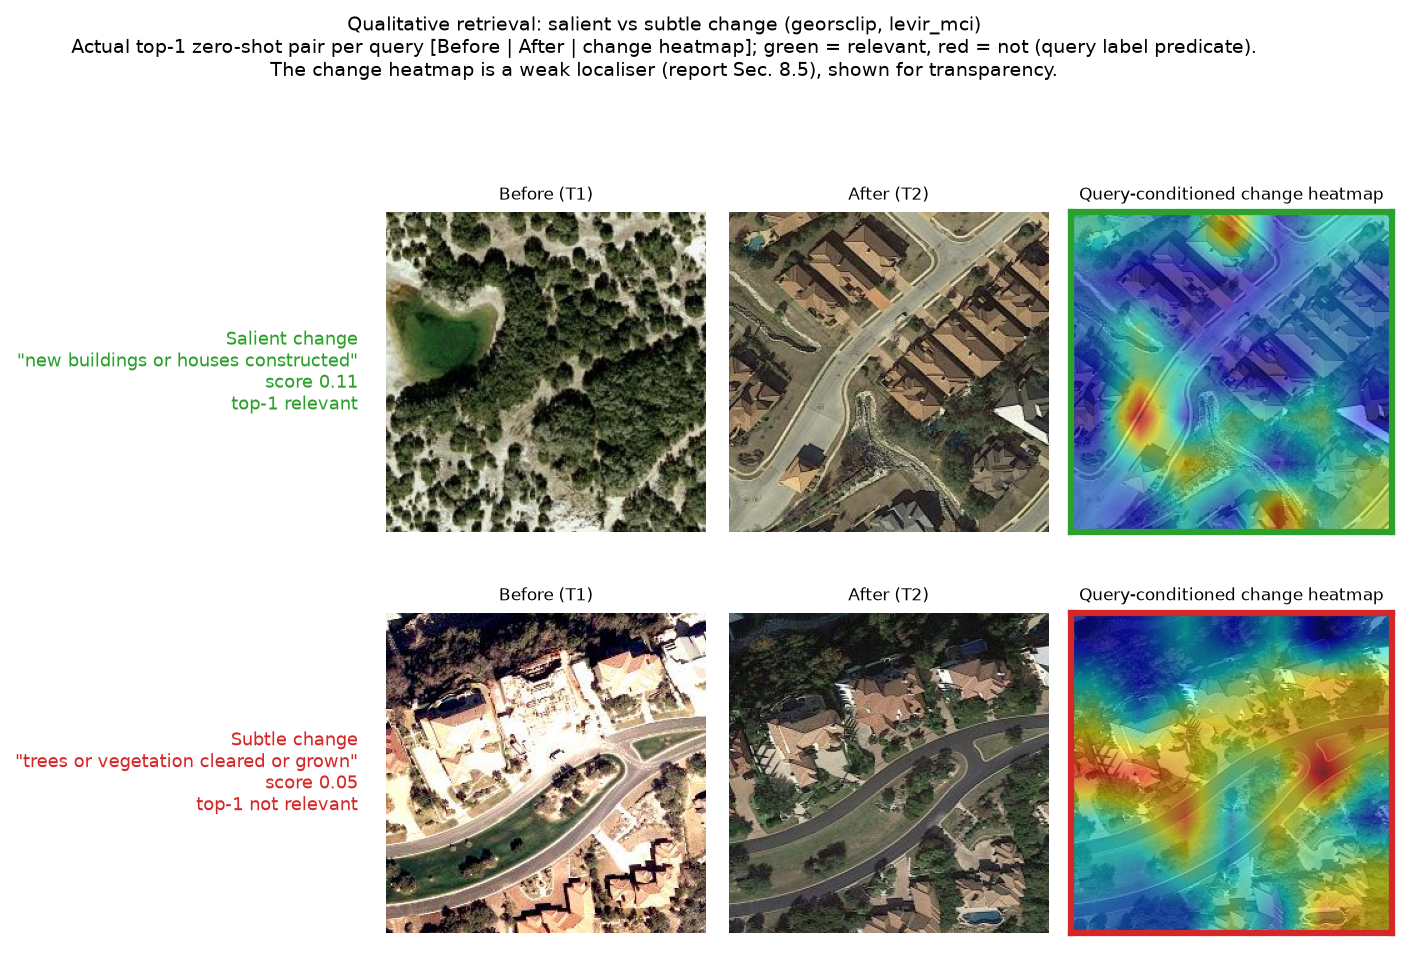
\includegraphics[width=\linewidth]{qualitative_examples__georsclip.png}
    \caption{The salience law in a single view (LEVIR-CC, GeoRSCLIP, zero-shot).
    For a salient query (new buildings) and a subtle one (vegetation), the panels
    show the engine's actual top-1 retrieved pair --- Before, After, and the
    query-conditioned change heatmap --- with a green border when that top-1
    satisfies the query's label predicate and red otherwise. The salient query
    retrieves a genuine construction event at rank~1, whereas the subtle query's
    top-1 is a false positive, mirroring the aggregate per-query AP of
    Figure~\ref{fig:saliencelaw}. Consistent with the localisation analysis
    (Table~\ref{tab:localization}), the change heatmap is only a weak localiser and
    is shown for transparency, not as a localisation result; the absolute
    $\Delta$-similarity scores (0.11 and 0.05) stay low, as expected under the
    frozen-VLM ceiling. Nothing is cherry-picked --- the figure regenerates
    deterministically from cached embeddings via
    \texttt{scripts/make\_qualitative\_figure.py}.}
    \label{fig:qualitative}
\end{figure}


\section{Resources and operational metrics}
\label{sec:resources}

All work fits the low-compute budget of the brief: a single laptop GPU, frozen
backbones, and cached embeddings. Tables~\ref{tab:hw}--\ref{tab:timings}
summarise hardware, model sizes, disk footprint and timings.

\begin{table}[H]
    \centering
    \caption{Hardware and software.}
    \label{tab:hw}
    \begin{tabular}{ll}
        \toprule
        \textbf{Item} & \textbf{Spec} \\
        \midrule
        GPU        & NVIDIA GeForce RTX 4060 Laptop, $\sim$8\,GB VRAM \\
        Runtime    & torch 2.10.0 + CUDA (cu130); CPU fallback supported \\
        OS / Python & Windows 11 / Python 3.12.10 \\
        Optional   & free Kaggle / Colab GPU for heavier sweeps \\
        \bottomrule
    \end{tabular}
\end{table}

\begin{table}[H]
    \centering
    \caption{Model sizes. The adapter is $<$0.2\% of the backbone - the PEFT premise.}
    \label{tab:models}
    \setlength{\tabcolsep}{4pt}
    \begin{tabular}{lrrr}
        \toprule
        \textbf{Model} & \textbf{Weights on disk} & \textbf{Params (approx)} & \textbf{Dim} \\
        \midrule
        CLIP ViT-L/14 (HF)                       & $\approx$1.71\,GB & $\approx$427\,M & 768 \\
        GeoRSCLIP (ViT-B/32 + RS5M ckpt)         & 605\,MB ckpt      & $\approx$151\,M & 512 \\
        RemoteCLIP (ViT-L/14 + ckpt)             & $\approx$1.7\,GB ckpt & $\approx$428\,M & 768 \\
        PEFT adapter (trainable part)   & 2.1--2.9\,MB      & 725{,}504 (768) / 528{,}128 (512) & - \\
        \bottomrule
    \end{tabular}
\end{table}

\begin{table}[H]
    \centering
    \caption{Disk footprint.}
    \label{tab:disk}
    \begin{tabular}{lr}
        \toprule
        \textbf{Component} & \textbf{Size} \\
        \midrule
        DEN archive (removable after extract)        & 7.09\,GB \\
        DEN extracted                                & 9.03\,GB \\
        CLIP weights cache (in-repo, gitignored)     & $\approx$1.6\,GB \\
        HF hub cache (in-repo, gitignored)           & $\approx$2.2\,GB \\
        Embedding caches (per encoder, 605 pairs)    & CLIP 3.76\,MB, GeoRSCLIP 2.52\,MB \\
        Trained adapters                             & 2.1--2.9\,MB each \\
        Total                               & $\approx$19.5\,GB ($\approx$12.5\,GB after deleting the archive) \\
        \bottomrule
    \end{tabular}
\end{table}

\begin{table}[H]
    \centering
    \caption{Timings (RTX 4060, dedicated timed pass).}
    \label{tab:timings}
    \begin{tabular}{lr}
        \toprule
        \textbf{Operation} & \textbf{Time} \\
        \midrule
        Retrieval scoring - numpy, 605 pairs, excl. text encode & 0.269\,ms/query \\
        End-to-end query - CLIP text forward + scoring, 605 pairs & 10.5\,ms \\
        Embedding precompute - CLIP L/14, $1024^2 \rightarrow 224$, GPU & 68\,ms/tile ($\approx$82\,s, one-time) \\
        PEFT training - 605 samples, 40 epochs, adapter only, GPU & $\approx$29\,s \\
        Fast test suite - mock encoders, CPU & $\approx$65\,s \\
        \bottomrule
    \end{tabular}
\end{table}


\section{Reproducibility}
\label{sec:repro}

Seeds are fixed; embeddings and adapters are cached and keyed by
(dataset, encoder, split, colour mode), with LoRA caches adding a \texttt{\_lora}
tag and cache invalidation on a pair-set change. The synthetic fixture is
regenerated automatically by the test suite. The commands below are the
reproducibility recipe used to produce the numbers in this report (a
step-by-step guide is in \texttt{README.md}).

{\footnotesize
\begin{verbatim}
pip install -e .
python -m scripts.download_den --dest data/DynamicEarthNet   # ~7 GB, one-time

# In-distribution: train on train split, evaluate on train/val/test
python -m scripts.run_pipeline --root data/DynamicEarthNet --encoder clip_vitl14 \
    --train-split train --eval-splits train val test --epochs 40
python -m scripts.run_pipeline --root data/DynamicEarthNet --encoder georsclip \
    --train-split train --eval-splits train val test --epochs 40
python -m scripts.run_pipeline --root data/DynamicEarthNet --encoder remoteclip \
    --train-split train --eval-splits train val test --epochs 40

# Best generalising config: GeoRSCLIP + NRG zero-shot (no PEFT training)
python -m scripts.run_pipeline --root data/DynamicEarthNet --encoder georsclip \
    --color-mode nrg --eval-splits train val test --skip-train

# NDVI / NRG colour-mode ablation (zero-shot only)
python -m scripts.run_pipeline --root data/DynamicEarthNet --encoder clip_vitl14 \
    --color-mode ndvi --eval-splits train val test --skip-train
python -m scripts.run_pipeline --root data/DynamicEarthNet --encoder georsclip \
    --color-mode ndvi --eval-splits train val test --skip-train
python -m scripts.run_pipeline --root data/DynamicEarthNet --encoder remoteclip \
    --color-mode nrg  --eval-splits train val test --skip-train

# LoRA adapter on visual encoder (GeoRSCLIP + NRG)
python -m scripts.run_pipeline --root data/DynamicEarthNet --encoder georsclip \
    --color-mode nrg --skip-train \
    --lora --lora-epochs 20 --lora-rank 4 --lora-alpha 8 \
    --eval-splits train val test

# Gradio UI
python -m src.app --root data/DynamicEarthNet --encoder clip_vitl14 --split train

# Fast suite (deterministic, no network)
pytest -q --ignore=tests/test_text_encoder.py
\end{verbatim}
}

The figures in this report are regenerated from cached embeddings (no GPU
training) via \texttt{scripts/\allowbreak{}export\_\allowbreak{}results.py} (writes one JSON per run +
\texttt{macro\_\allowbreak{}summary.csv}) followed by \texttt{scripts/\allowbreak{}make\_\allowbreak{}figures.py} and
\texttt{scripts/\allowbreak{}make\_\allowbreak{}comparison\_\allowbreak{}figure.py}. The main sources of run-to-run
variance are GPU non-determinism in the encoders and the random partitions of the
cross-validation; the cross-validation means and standard deviations reported
throughout quantify the latter, and seeds are fixed for the former.

\paragraph{Code, data, and demonstration availability.}
The full source, the preprocessed-data download recipe, the trained adapters, and
the committed benchmark results are available in the public repository at
\url{https://github.com/Panagiotis427/MSc_GBDA-OV_Temporal_Change_Retrieval}. The
Gradio search engine is deployed and publicly usable, over a bundled synthetic
corpus, at
\url{https://huggingface.co/spaces/panagiotis427/Open_Vocabulary_Temporal_Change_Retrieval};
five short screen-recorded walkthroughs of the interface, in the repository's
\texttt{demos/} directory, show the engine in use end to end.


\section{Limitations and future work}
\label{sec:future}

The limitations group by how much they bound the conclusions. The first tier
concerns credibility: all mAP figures use LULC-derived pseudo-labels rather than
human-annotated query relevance, so a true information-retrieval benchmark would
require collecting human relevance judgements, the single change that would most
strengthen the evaluation. The second tier concerns the method: supervision is
weak (captions are derived from dominant-class label flips), so LLM-generated or
human-written change captions are a natural improvement; both the ProjectionHead
and LoRA adapters overfit train-AOI statistics, so multi-AOI held-out training or
domain-randomised augmentation might close the out-of-distribution gap; and
Sentinel-1~\cite{sentinel1}/2~\cite{sentinel2} fusion is unimplemented, though
\texttt{aoi\_metadata.json} confirms 51/75 AOIs carry full SAR (S1) coverage and
feeding SAR $\Delta$-features would be a direct extension of the NRG pattern. The
third tier concerns scope: crop-precise polygon grounding for finer localisation
remains open --- the QFabric pentatemporal five-date imagery with polygon
change-masks is the natural vehicle for it, but that source is currently
access-gated; fMoW is wired only at the protocol level with no concrete loader;
and a learned query-to-patch attention head is unexplored because every trained
head on this data memorises rather than generalises.


\section{Conclusion}
\label{sec:conclusion}

The system fulfils the GBDA Lab Project's brief: an open-vocabulary, frozen-backbone change
search engine with a Gradio interface, a label-grounded Recall@$K$/mAP benchmark,
seasonal-vs-permanent error analysis, temporal pinpointing of the change within each
AOI timeline (Appendix~\ref{sec:temporalpinpoint}), and a clear zero-shot vs PEFT
comparison across three CLIP-variant encoders on Dynamic EarthNet, reported under a
strict statistical protocol. Four findings emerge. First, a learned adapter shows no
out-of-distribution gain: the large in-distribution PEFT lift
($0.043 \rightarrow 0.420$, up to 0.999 on QFabric) is the adapter scored on its
own training pairs (memorisation), and under the headline GeoRSCLIP+NRG
configuration leakage-free cross-validated PEFT ($0.196 \pm 0.049$) merely
overlaps frozen zero-shot ($0.139 \pm 0.024$) within fold variance, so low-compute
fine-tuning is not shown to help retrieval out of distribution. Second, out of
distribution the frozen zero-shot wins, but weakly: the GeoRSCLIP+NRG estimate is
$0.100 \pm 0.139$ under 5-fold AOI cross-validation (the single-split 0.426 is a
high-variance fold), so RS pre-training and NIR false-colour help, but the
absolute signal is small. Third, the recoverable signal is a matter of evaluation
and method, not bad data: pixel-fraction relevance makes 9/10 change-types
evaluable and a localised patch-level scorer lifts cross-validated mAP to
$0.193$, making construction change (new buildings, urban expansion) retrievable
above chance, with only snow genuinely absent from the data. Fourth, LoRA does
not close the gap either (every rank/epoch overfits to test $\approx$0.07),
consistent with the adapters-only-memorise finding.

The deliverable's value is the motivated, honestly-audited comparison, not a
single best number: spectral physics and spatial locality carry the weak signal
that exists, global embeddings and learned visual priors dilute or memorise it,
and small single-split scores require cross-validation before they estimate
generalisation. Across all four datasets the recovered signal tracks change
salience (Figure~\ref{fig:saliencelaw}): weak on DEN's subtle spectral
transitions, dataset-dependent on QFabric, strong on LEVIR-CC's salient
building/road change (per-query AP $\approx$0.6--0.8) yet near-random on its
subtle vegetation and sparse water, and - on SECOND-CC's seven-query open
vocabulary - above every prevalence floor but only modestly (zero-shot macro
$\approx$0.33). Localising the change (LEVIR-MCI/SECOND-CC masks) is weaker still:
the heatmap clears its random-patch floor by at most $\approx$0.04--0.10. The same
regularity governs the temporal axis (Appendix~\ref{sec:temporalpinpoint}): sharp,
visually distinct events such as snow melt are pinpointed in time above chance,
whereas gradual transitions such as deforestation collapse toward the random
floor -- so change salience sets the recoverable signal in time as well as in
space and vocabulary.


\clearpage
\phantomsection
\addcontentsline{toc}{section}{References}
\bibliographystyle{ieeetr}
\bibliography{references}

\begin{appendices}

\clearpage
\section[Native 3 m raster source: data-source fidelity]{Native 3\,m raster source: data-source fidelity}
\label{sec:nativeraster}

The primary evaluation uses the $\sim$7\,GB preprocessed RGB/NIR-JPEG DEN subset
in preference to the $\sim$525\,GB raw mirror. To confirm that this pragmatic
choice does not cost retrieval performance - i.e.\ that the conclusions survive
at full radiometric depth - the adapter was also run directly on the native
Planet-Fusion~\cite{planetfusion} surface-reflectance rasters
($1024\times1024\times4$ \texttt{int16}, Blue/Green/Red/NIR, 3\,m), read in-memory
from the per-zone \texttt{planet.<UTM>.zip} archives with no lossy re-encoding,
yielding 23 labelled AOIs (552 change pairs, under that earlier pipeline's denser pairing) spanning all seven DEN
land-cover classes. The adapter (frozen CLIP ViT-L/14, \texttt{difference} change
feature) was scored under the same held-out protocol as
Section~\ref{sec:denmain}: a 5-seed stratified AOI-level hold-out (split on real
cube id, stratified by dominant change class), reporting mean $\pm$ std across
seeds. These particular figures were produced by an earlier iteration of this
project's codebase (the \texttt{cross\_validate.py} pipeline over
\texttt{train\_v2.py} and \texttt{evaluate\_v2.py}), which is not part of the
committed source; the run is therefore a one-off that cannot be regenerated from the
current tree. The per-seed fold values are archived verbatim in
\texttt{results/cv\_eval\_\_clip\_vitl14\_\_rgb\_\_planet3m.json}, and the
reproducible native-3m counterpart --- run through this repository's own committed
\texttt{cv\_eval} harness --- is reported in Table~\ref{tab:native3mcv}. The adapter
table below is retained for the source-fidelity comparison it supports, read with
that provenance caveat in mind.

\begin{table}[H]
    \centering
    \caption{Native 3\,m raster source (CLIP ViT-L/14, adapter, \texttt{difference};
    23 AOIs, 5-seed stratified AOI cross-validation). NIR here is the
    NIR-Red-Green false colour (matching \texttt{nrg} elsewhere). These figures come
    from a one-off run on the full-resolution Planet-Fusion rasters, external to the
    committed \texttt{results/} artifacts (which cover the $\sim$7\,GB JPEG subset);
    its generating pipeline is not committed, so these figures are not reproducible
    from the tree (per-seed values archived in the run's JSON). Reported for the
    source-fidelity comparison only; reproducible counterpart in
    Table~\ref{tab:native3mcv}.}
    \label{tab:nativeraster}
    \begin{tabular}{llc}
        \toprule
        \textbf{Configuration} & \textbf{colour} & \textbf{mAP (mean $\pm$ std)} \\
        \midrule
        Adapter                & RGB  & 0.236 $\pm$ 0.030 \\
        Adapter                & NIR (NRG)  & 0.253 $\pm$ 0.040 \\
        Adapter, class-weighted & RGB & 0.265 $\pm$ 0.029 \\
        Adapter, $2\times2$ patch tiling & RGB & 0.202 $\pm$ 0.022 \\
        \bottomrule
    \end{tabular}
\end{table}

Two readings follow, both consistent with the JPEG-subset audit. First, the native
rasters land in the same band as the preprocessed subset under cross-validation
(cf.\ the audited CV figures in Section~\ref{sec:denmain}): full \texttt{int16}
radiometric depth and the intact NIR channel buy no material retrieval gain over
the $\sim$7\,GB RGB/NIR-JPEG subset, so the data-source choice in
Section~\ref{sec:data} is vindicated - the bottleneck is the frozen
web-pretrained features and the small labelled AOI set, not imagery compression.
Second, no full-tile configuration is statistically separable from another: RGB
($0.236\pm0.030$), NRG ($0.253\pm0.040$) and per-class loss weighting
($0.265\pm0.029$) all overlap within one standard deviation, and the $+0.017$
NRG-over-RGB margin sits well inside that noise - the same null result as the
colour-mode ablation (Section~\ref{sec:ablations}), where the large single-split
NRG lift is a high-variance fold. Only $2\times2$ patch tiling separates, and
downward ($0.202\pm0.022$): splitting the 1024-px tile discards the CLIP global
spatial context. RGB at the native tile scale is the simplest configuration in the
indistinguishable top group and remains the reference.

\paragraph{Cross-check under the repository's own benchmark.}
The table above reports the fitted adapter under a 5-seed stratified AOI hold-out.
As a second, independent check --- this time zero-shot and under the
disjoint 5-fold AOI \texttt{cv\_eval} harness that produced the JPEG-subset
headline (dominant-class relevance over the ten DEN queries;
Section~\ref{sec:denmain}), via the registry-resolved
\texttt{dynamic\_earthnet\_planet} loader --- the native rasters were scored
directly against the preprocessed subset. Both use the same dominant-class
relevance metric, so the two rows are read as adapter-vs-zero-shot, not
metric-vs-metric. Table~\ref{tab:native3mcv} reports the head-to-head. Under the
identical encoder, metric and zero-shot setting the native 3\,m source (macro mAP
$0.130\pm0.068$) sits at or above the JPEG subset ($0.076$; $0.123$ under
fraction relevance), despite covering fewer AOIs. The comparison is not fully
controlled --- the corpora differ in AOI count (23 vs 75) and colour composite
(native RGB vs JPEG NRG) --- but for this corpus colour barely moves the score
(georsclip: RGB $0.085$ vs NRG $0.100$), so the direction is robust: the native
source is no worse, corroborating the no-loss conclusion of
Section~\ref{sec:data} under the repository's own zero-shot cross-validated
benchmark rather than the fitted hold-out above.\footnote{The
leakage-free $k$-fold PEFT estimate on the native rasters is $0.215\pm0.306$; the
large variance (one fold at $0.75$, the rest $0.03$--$0.19$, driven by few positives
per small fold) makes the zero-shot figure the reliable point of comparison.}
The two native-source adapter estimates also diverge sharply in stability --- the
external hold-out's tight $0.236\pm0.030$ (Table~\ref{tab:nativeraster}) against the
leakage-free \texttt{cv\_eval} adapter's $0.215\pm0.306$ --- so the fitted-adapter
level is not read as a gain over zero-shot: the instability under leakage-free folds
is exactly the behaviour Section~\ref{sec:memorisation} attributes to adapter
memorisation on this small labelled corpus, and the source-fidelity reading
accordingly rests on the stable, reproducible zero-shot rows.

\begin{table}[H]
    \centering
    \caption{Native 3\,m rasters vs the preprocessed JPEG subset under the
    repository's own \texttt{cv\_eval} benchmark (CLIP ViT-L/14, 5-fold AOI
    cross-validation, zero-shot, dominant-class relevance unless noted).}
    \label{tab:native3mcv}
    \begin{tabular}{llc}
        \toprule
        \textbf{Source} & \textbf{colour} & \textbf{macro mAP (mean $\pm$ std)} \\
        \midrule
        Native 3\,m raster & RGB & 0.130 $\pm$ 0.068 \\
        JPEG subset                    & NRG & 0.076 \\
        JPEG subset (fraction rel.)    & NRG & 0.123 \\
        \bottomrule
    \end{tabular}
\end{table}

\paragraph{Controlled compression and resolution ablation.}
The cross-checks above leave two confounds (AOI count and colour composite). To
isolate image fidelity itself, everything is held fixed --- the same 23 AOIs, 253
pairs, RGB composite, encoder, zero-shot scoring and 5 AOI folds --- and only the
degradation applied to each tile before encoding is varied. The native lossless
raster is the upper bound; every other row is the identical corpus pushed through a
lossy round-trip in memory. Relevance labels (from the lossless masks) and the
text-query vectors are computed once and shared across all rows, so the only thing
that changes between rows is the image. Two degradation families are swept: JPEG~\cite{jpeg}
quality $q\in\{95,75,50,25,10\}$ (radiometric / compression loss at full
resolution), and bicubic downsampling to $\{512,256,128,64\}$\,px followed by JPEG
$q{=}75$ (the resolution loss the preprocessed subset's resize step would
introduce). Table~\ref{tab:jpegablation} and Figure~\ref{fig:jpegablation} report
CLIP ViT-L/14.

\begin{table}[H]
    \centering
    \caption{Controlled degradation ablation on the native 3\,m rasters (CLIP
    ViT-L/14, RGB, zero-shot, 253 pairs / 23 AOIs, 5-fold AOI cross-validation,
    seed 42). Identical corpus throughout; only the per-tile degradation varies.
    Every row overlaps native within one fold standard deviation.}
    \label{tab:jpegablation}
    \begin{tabular}{lcc}
        \toprule
        \textbf{Degradation} & \textbf{macro mAP (mean $\pm$ std)} & \textbf{$\Delta$ vs native} \\
        \midrule
        Native 3\,m (lossless, 1024\,px) & 0.130 $\pm$ 0.068 & --- \\
        \midrule
        JPEG $q{=}95$  & 0.115 $\pm$ 0.065 & $-0.015$ \\
        JPEG $q{=}75$  & 0.094 $\pm$ 0.064 & $-0.036$ \\
        JPEG $q{=}50$  & 0.128 $\pm$ 0.078 & $-0.001$ \\
        JPEG $q{=}25$  & 0.095 $\pm$ 0.065 & $-0.034$ \\
        JPEG $q{=}10$  & 0.138 $\pm$ 0.108 & $+0.009$ \\
        \midrule
        Downsample 512\,px ($+$ JPEG $q75$) & 0.088 $\pm$ 0.054 & $-0.042$ \\
        Downsample 256\,px & 0.154 $\pm$ 0.150 & $+0.025$ \\
        Downsample 128\,px & 0.146 $\pm$ 0.166 & $+0.016$ \\
        Downsample \phantom{0}64\,px & 0.216 $\pm$ 0.213 & $+0.086$ \\
        \bottomrule
    \end{tabular}
\end{table}

\begin{figure}[H]
    \centering
    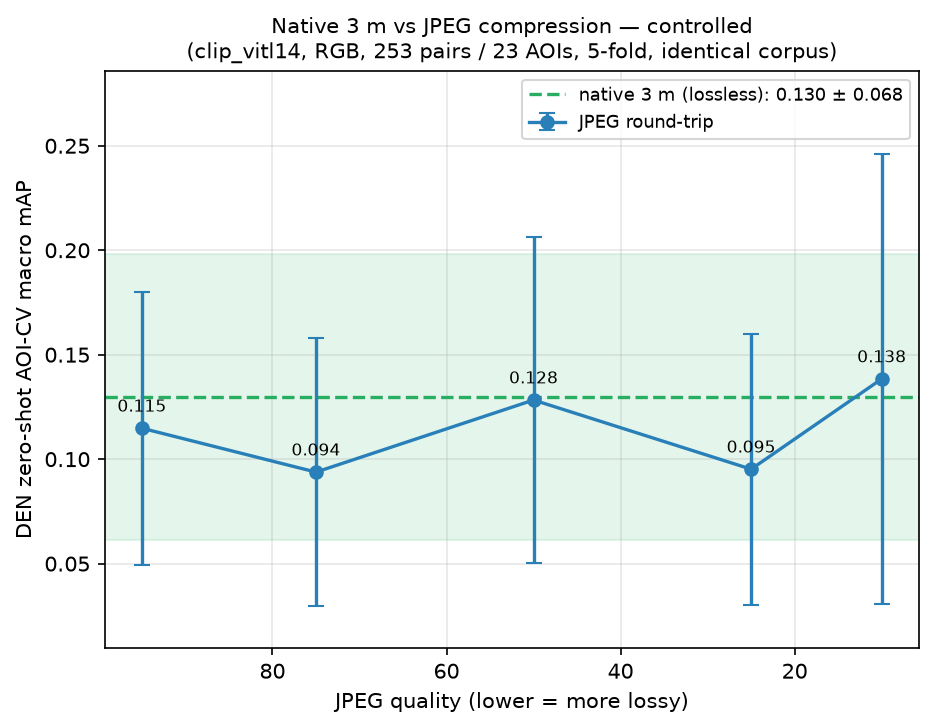
\includegraphics[width=0.72\linewidth]{jpeg_ablation__clip_vitl14__rgb.png}
    \caption{Zero-shot AOI-CV macro mAP versus JPEG quality on the identical native
    corpus (CLIP ViT-L/14, RGB). The dashed line and shaded band are the native
    lossless mean $\pm$ fold std. Every JPEG point sits inside the band, and the
    curve is non-monotonic --- the most-compressed setting ($q{=}10$) scores above
    the lightly-compressed ones --- so the variation is fold sampling, not a
    compression effect.}
    \label{fig:jpegablation}
\end{figure}

The reading is unambiguous: image fidelity is not the bottleneck. The largest gap
from native across the entire JPEG sweep is $0.036$\,mAP --- about half of one
fold's standard deviation ($\sim$$0.065$) --- and the deltas alternate sign with
quality, so they are fold-sampling noise rather than a degradation signal. The
resolution sweep is, if anything, more decisive: collapsing the tile to 64\,px (a
$16\times$ linear reduction) does not lower retrieval and nominally raises it,
because the frozen encoder resizes every input to its own $224$\,px window and the
change signal that survives in the global embedding is coarse --- high-frequency
spatial detail is simply not what the web-pretrained features exploit for these
queries.\footnote{The honest caveat is that fold variance grows under aggressive
downsampling (std up to $0.21$ at 64\,px, driven by few positives per small fold),
so the claim is only that no degradation is detectable at this corpus size, not
exact equivalence.} This is direct evidence for the report's central thesis
(Section~\ref{sec:denmain} and Appendix~\ref{sec:nativeraster}): the ceiling is the frozen
web-pretrained representation and the small labelled-AOI set, not imagery
compression or resolution. It also retroactively vindicates the
Section~\ref{sec:data} decision to work from the $\sim$7\,GB preprocessed subset
rather than the $\sim$525\,GB native mirror.

The result is not an artefact of the generic web-pretrained encoder. Repeating the
identical ablation with the RS-pretrained GeoRSCLIP (ViT-B/32) gives the same null
(Table~\ref{tab:jpegablationgeors}): the largest deviation from its native baseline
($0.085\pm0.059$) is $0.027$\,mAP, again inside one fold standard deviation, and
every JPEG and downsample row overlaps native. Tellingly, the two encoders disagree
on the sign of the small downsampling deltas --- CLIP nominally rises toward
64\,px, GeoRSCLIP nominally falls --- which is exactly what fold-sampling noise, and
not a real fidelity effect, would produce. Both the domain-agnostic and the
RS-domain backbone are insensitive to compression and resolution on this task.

\begin{table}[H]
    \centering
    \caption{Confirmation under GeoRSCLIP (ViT-B/32, RGB, zero-shot, same 253
    pairs / 23 AOIs, 5-fold AOI cross-validation, seed 42). Same null as
    Table~\ref{tab:jpegablation}: every row within one fold standard deviation of
    native.}
    \label{tab:jpegablationgeors}
    \begin{tabular}{lcc}
        \toprule
        \textbf{Degradation} & \textbf{macro mAP (mean $\pm$ std)} & \textbf{$\Delta$ vs native} \\
        \midrule
        Native 3\,m (lossless, 1024\,px) & 0.085 $\pm$ 0.059 & --- \\
        \midrule
        JPEG $q{=}95$  & 0.083 $\pm$ 0.054 & $-0.002$ \\
        JPEG $q{=}75$  & 0.095 $\pm$ 0.075 & $+0.010$ \\
        JPEG $q{=}50$  & 0.091 $\pm$ 0.058 & $+0.006$ \\
        JPEG $q{=}25$  & 0.091 $\pm$ 0.073 & $+0.006$ \\
        JPEG $q{=}10$  & 0.104 $\pm$ 0.079 & $+0.019$ \\
        \midrule
        Downsample 512\,px ($+$ JPEG $q75$) & 0.102 $\pm$ 0.082 & $+0.017$ \\
        Downsample 256\,px & 0.076 $\pm$ 0.059 & $-0.010$ \\
        Downsample 128\,px & 0.074 $\pm$ 0.075 & $-0.011$ \\
        Downsample \phantom{0}64\,px & 0.058 $\pm$ 0.035 & $-0.027$ \\
        \bottomrule
    \end{tabular}
\end{table}

\clearpage
\section{Temporal pinpointing: when does the change occur?}
\label{sec:temporalpinpoint}

The project brief singles out Dynamic EarthNet for its ability to ``pinpoint exact
time-steps of change'' and asks evaluation to verify that the model identifies ``the
specific temporal window where the change was most prominent compared to stable
time-steps''. The retrieval metrics so far answer which pair shows a change (ranking
across AOIs); this is the orthogonal question of when a change happens (ranking
time-steps within one AOI's timeline), and it is uniquely accessible through the
native loader's monthly raster stack. The loader is built with monthly pairing so
each AOI's consecutive pairs form its 24-month timeline; the per-step change score
is the same zero-shot $\Delta$-similarity used throughout
($\cos(q,f_t)-\cos(q,f_{t-1})$); a step is relevant when the query predicate fires
on its monthly transition label. Within each AOI the steps are ranked and the
ranking is scored by average precision (a per-AOI temporal AP), and the peak-hit
rate is reported --- whether the single highest-scoring step is a true transition,
at exact and $\pm1$-month tolerance. Significance uses a permutation test that
shuffles relevance within each AOI (preserving its step count) plus BH-FDR.

\begin{table}[H]
    \centering
    \caption{Temporal pinpointing on native 3\,m DEN (CLIP ViT-L/14, RGB,
    zero-shot): ranking the monthly steps within each AOI timeline. ``peak $\pm$1''
    is the fraction of AOIs whose top-scored step is within one month of a true
    transition. Macro temporal mAP 0.309 vs a 0.207 permutation floor.}
    \label{tab:temporalpinpoint}
    \begin{tabular}{lccccc}
        \toprule
        \textbf{Query} & \textbf{temporal mAP} & \textbf{rand} & \textbf{peak $\pm$1mo} & \textbf{perm $p$} & \textbf{AOIs} \\
        \midrule
        seasonal snow melting away      & 0.586 & 0.200 & 1.00 & 0.025 & 2 \\
        bare soil or land cleared       & 0.324 & 0.214 & 0.57 & 0.067 & 7 \\
        forest loss                     & 0.273 & 0.193 & 0.40 & 0.160 & 5 \\
        new water body or flooding      & 0.221 & 0.246 & 1.00 & 0.409 & 1 \\
        deforestation, forest $\to$ soil & 0.142 & 0.183 & 0.20 & 0.617 & 5 \\
        \midrule
        \textbf{macro}                  & \textbf{0.309} & 0.207 & 0.63 & --- & --- \\
        \bottomrule
    \end{tabular}
\end{table}

\begin{figure}[H]
    \centering
    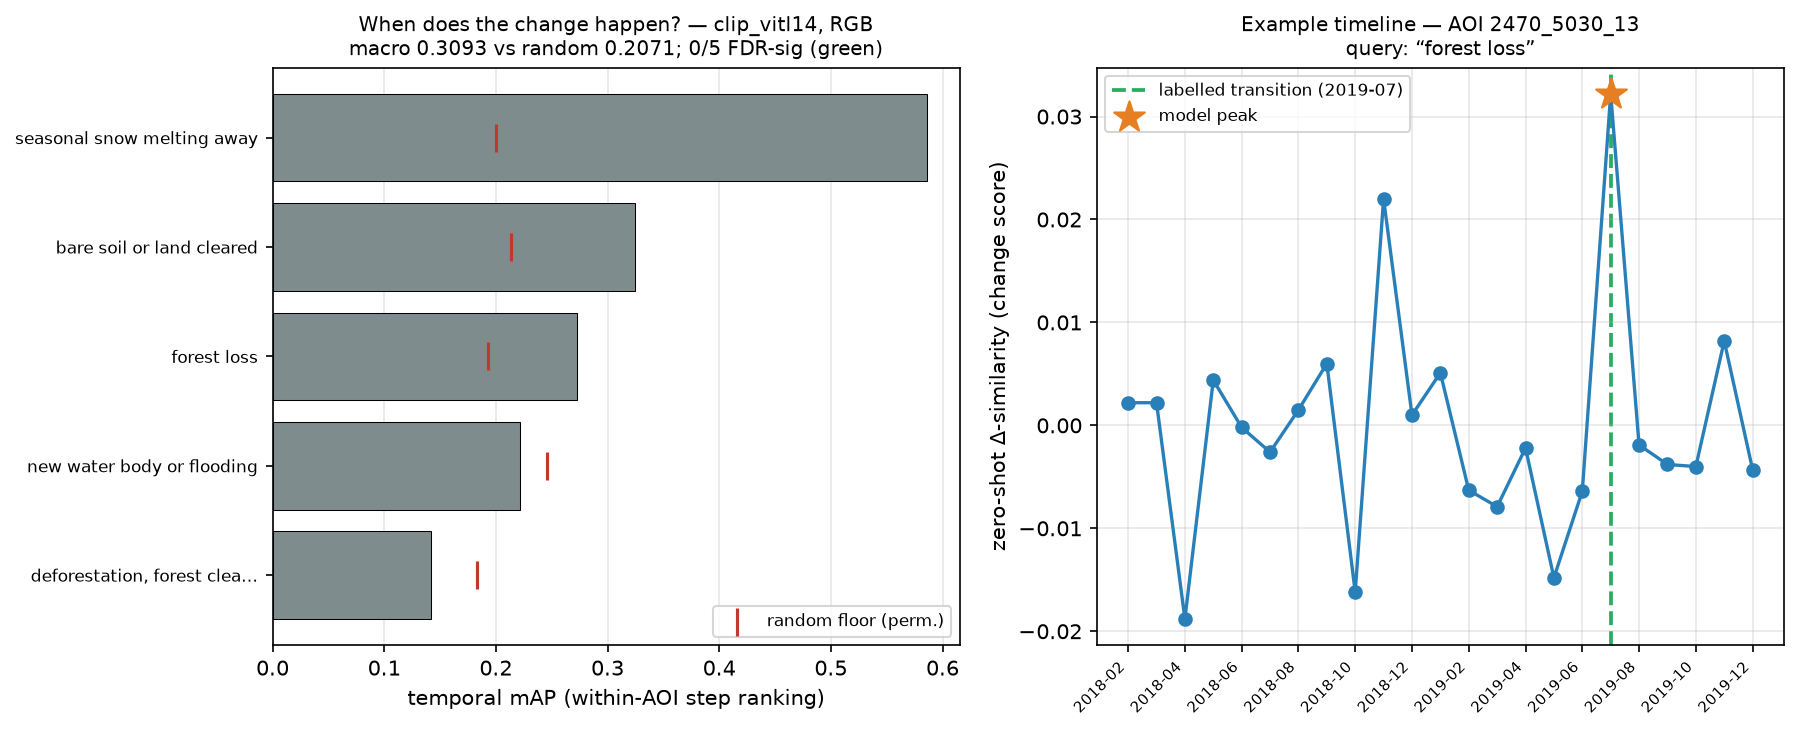
\includegraphics[width=\linewidth]{temporal_pinpoint__clip_vitl14__rgb.png}
    \caption{Left: per-query temporal mAP (within-AOI step ranking) against the
    permutation random floor (red ticks). Right: an example AOI timeline --- the
    zero-shot change score for ``forest loss'' spikes at the labelled transition
    month (2019-07, dashed green), where the model's peak (orange star) also lands.}
    \label{fig:temporalpinpoint}
\end{figure}

The system does locate change in time above chance: macro temporal mAP $0.309$
against a $0.207$ random floor, and within a $\pm1$-month tolerance the model's peak
step lands on a true transition $63\%$ of the time
(Table~\ref{tab:temporalpinpoint}, Figure~\ref{fig:temporalpinpoint}). The signal
is strongest for temporally sharp events --- snow melt ($0.586$, $p=0.025$) and
abrupt soil clearing ($0.324$) --- and weak for gradual or ambiguous ones
(deforestation $0.142$, below its floor). As with spatial localization
(Section~\ref{sec:localization}) the effect is encoder-dependent: repeating the
study with GeoRSCLIP (ViT-B/32) gives macro $0.146$ vs the same $0.207$ floor --- at
or below chance --- so the larger general-purpose ViT-L/14 pinpoints change in time
where the smaller RS-pretrained backbone does not. The honest limit is statistical
power: only 1--7 AOIs carry positives per query, so although the aggregate clears
the floor and snow melt is individually significant at $p=0.025$, no query survives
BH-FDR --- the same small-labelled-AOI ceiling documented throughout. Pinpointing
when a change occurs is feasible for salient, abrupt transitions on a capable frozen
encoder, but, like pinpointing where, it is harder than retrieving whether the
change is present.

\clearpage
\section{Post-retrieval re-ranking}
\label{sec:rerank}

The Gradio app exposes two optional, per-query re-ranking toggles. Both are
evaluated on the held-out test split (110 pairs, 3 queries with positives) using
GeoRSCLIP + NRG zero-shot (Table~\ref{tab:rerank}).

\begin{table}[H]
    \centering
    \caption{Re-ranking on the test split (GeoRSCLIP + NRG, zero\_shot). Both
    strategies reduce retrieval quality. Best per column in bold.}
    \label{tab:rerank}
    \begin{tabular}{lccccc}
        \toprule
        \textbf{Strategy} & \textbf{R@1} & \textbf{R@3} & \textbf{R@5} & \textbf{R@10} & \textbf{mAP} \\
        \midrule
        baseline (no rerank) & 0.133 & \textbf{0.333} & \textbf{0.400} & \textbf{0.467} & \textbf{0.426} \\
        diversity            & 0.133 & 0.267 & 0.267 & 0.267 & 0.344 \\
        coherence            & 0.133 & 0.200 & 0.267 & 0.467 & 0.339 \\
        \bottomrule
    \end{tabular}
\end{table}

Both strategies reduce retrieval quality: diversity deduplicates locations,
pushing relevant pairs from the same AOI out of the top window; coherence clusters
geographically near the top-1 result, but relevant pairs are globally distributed.
Neither optimises semantic relevance - they trade mAP ($-0.082$ diversity,
$-0.087$ coherence) for display properties (result variety and spatial coherence),
and are exposed as optional toggles alongside a continental geographic filter
driven by \texttt{aoi\_metadata.json}.

\end{appendices}

\end{document}
